\documentclass[reprint,amsmath,amssymb,aps,nofootinbib]{revtex4-2}

\usepackage{graphicx}
\usepackage{bm}
\usepackage{mathtools}
\usepackage{mathrsfs}
\usepackage{amsthm}
\usepackage{bbm}
\usepackage{hyperref}
\usepackage{microtype}

\hypersetup{colorlinks=true,citecolor=blue,linkcolor=blue,urlcolor=blue}

\newtheorem{definition}{Definition}
\newtheorem{theorem}{Theorem}
\newtheorem{proposition}{Proposition}
\newtheorem{lemma}{Lemma}
\newtheorem{corollary}{Corollary}
\newtheorem{remark}{Remark}
\newtheorem{assumption}{Assumption}

\newcommand{\Tr}{\operatorname{Tr}}
\newcommand{\supp}{\operatorname{supp}}
\newcommand{\id}{\mathbbm{1}}
\newcommand{\Lag}{\mathcal L}
\newcommand{\E}{\mathbb E}
\newcommand{\F}{\mathfrak F}
\newcommand{\FreeOps}{\mathfrak O}
\newcommand{\R}{\mathsf R}
\newcommand{\Chan}{\mathsf{Chan}}
\newcommand{\Proc}{\mathsf{Proc}}
\newcommand{\Free}{\mathrm{free}}
\newcommand{\rev}{\mathrm{rev}}
\newcommand{\Ddiamond}{D_{\diamond}}
\newcommand{\Rrob}{R_{\rm rob}}
\newcommand{\Rlyap}{R_{\rm Lyap}}
\newcommand{\Rdyn}{R_{\rm dyn}}
\newcommand{\GBZ}{\mathrm{GBZ}}
\newcommand{\NHSE}{\mathrm{NHSE}}
\newcommand{\HN}{\mathrm{HN}}
\newcommand{\Damp}{D_{\rm amp}}
\newcommand{\Qexp}{\mathfrak Q_{\exp}}
\newcommand{\diag}{\operatorname{diag}}

\begin{document}

\preprint{APS/123-QED}

\title{A Quantum Resource Theory for the Reciprocity-Breaking Sector of the Non-Hermitian Skin Effect via Quantum Channels}

\author{Ann Author}
\affiliation{Authors' institution and/or address}

\date{\today}

\begin{abstract}
We formulate a quantum resource theory for the transpose-reciprocity-breaking sector of the
non-Hermitian skin effect (NHSE), with fixed-time CPTP channels as the primitive resource
objects. A non-Hermitian propagator is embedded into a reciprocity-compatible Julia unitary
dilation, while a Hamiltonian trajectory is treated as a derived family of channel resources.
The free objects are reciprocal quasi-local channels and the free transformations are
physically realizable reciprocity-covariant superchannels. The resulting preorder has two
faithful monotones, the channel asymmetry $A_\diamond$ and generalized robustness $\Rrob$.
We separate four logically distinct results. First, on the uniform Hatano--Nelson gauge
orbit, an exact two-site calibration gives a closed formula for $A_\diamond$ and proves a
fixed-time no-go: no deterministic free superchannel can implement the universal gauge
amplification $g\mapsto\eta g$ with $\eta>1$. Second, while the \emph{global} monotones
$A_\diamond,\Rrob$ of a single fixed-time channel are bounded by one and have vanishing
tensor-power rate, we show that this bound is specific to that global, indivisible-channel
construction: restricting to the physically natural class of spatially local free
superchannels (the analogue of LOCC in entanglement theory) yields an exactly additive,
genuinely extensive resource density, computed in closed form on the Hatano--Nelson orbit and
verified numerically, including its approximate survival under the quasi-local coupling of a
genuinely translation-invariant chain. Third, thermodynamic persistence still has no universal
quantitative relation to the skin length $1/|g|$: rescaling the energy scale changes the
persistent channel asymmetry while leaving the GBZ radius unchanged, a distinct obstruction
that extensivity alone does not remove. Fourth, the necessity theorem is presented as a
dictionary lemma rather than the main conceptual result, and the winding-cancellation
counterexample shows that a single scalar topological invariant cannot serve as a complete
multichannel witness. Clean reciprocity forces zero determinant winding and reciprocal roots,
and reciprocal disordered chains obey exact Lyapunov pairing. The resulting picture is a
compact channel QRT with explicit operational obstructions, an extensive block-additive
resource density, a controlled thermodynamic no-go, and a sharp hierarchy of spectral,
spatial, and dynamical diagnostics. \emph{This revision} additionally (i) generalizes the
whole architecture to a symmetry-extended framework applicable to any covariant involution
satisfying four structural axioms, of which the transpose sector is one instance; (ii) proves
that the spatial-locality restriction underlying extensivity is a definitional necessity
rather than a technical convenience, on the same footing as the LOCC restriction in
entanglement theory; (iii) introduces a time-optimized channel resource that is exactly
invariant under the energy rescaling responsible for the thermodynamic-persistence
obstruction, and gives it a nondegenerate lower bound on the Hatano--Nelson orbit; (iv)
upgrades the coupled-chain extensivity claim from a numerical proof sketch to a proven
approximate-monotonicity bound with an explicit, exponentially small error; and (v) proves
that the block-additive resource is a complete NHSE witness on cellular multiband arrays,
explaining why it does not fall to the winding-cancellation counterexample that defeats the
scalar topological invariant.
\end{abstract}

\maketitle

%===============================================================
\section{Operational starting point: fixed-time NHSE channels as resources}
\label{sec:operational}

A resource theory is specified by a class of objects, a free subset, physically
admissible free transformations, and the resulting conversion preorder; resource monotones are
then functions nonincreasing under that preorder
\cite{ChitambarGour,LiuWinter,LiuYuan}. In channel resource theories, the objects are
quantum channels and the transformations are quantum superchannels
\cite{LiuWinter,LiuYuan,ChiribellaSupermap}.

Our aim is to formulate a QRT in which transpose-reciprocity breaking is the channel
resource that underlies the reciprocity-breaking sector of the NHSE. The primitive
resource object is a CPTP channel at a fixed operational time $t$. A time-dependent
non-Hermitian evolution gives a family of such resource objects,
but that family is a derived process trajectory rather than a new primitive object.
This distinction keeps the resource-theoretic layer standard while allowing spectral,
spatial, and dynamical NHSE diagnostics to be attached to the same trajectory.

A non-Hermitian Hamiltonian by itself does not define a CPTP map. We therefore embed its
normalized propagation into a unitary dilation whose transpose symmetry is exactly
compatible with the reciprocity used below. The dilation is an operational embedding,
not a claim that every physical open-system realization of NHSE is equivalent to a
postselected non-Hermitian Hamiltonian.

\begin{definition}[Single-particle Hilbert space]
For a chain of length $L$ with internal dimension $M$, let

$$
\mathcal H_L=\operatorname{span}\{|n,\alpha\rangle:
1\le n\le L,\ 1\le\alpha\le M\}.
$$

The spatial basis is fixed once and for all. All reciprocity statements below refer
to this basis.
\end{definition}

\begin{definition}[Admissible normalized propagator]
\label{def:normcontr}
Let $H$ be a finite-dimensional non-Hermitian Hamiltonian and

$$
U_H(t)=e^{-iHt}.
$$

Let $\mathcal H_{\rm adm}$ be a prescribed Hamiltonian class such that

$$
\sup_{H\in\mathcal H_{\rm adm}}\|U_H(t)\|_\infty<\infty
$$

for every operational time $t$. Define

$$
\kappa_*(t)=\sup_{H\in\mathcal H_{\rm adm}}\|U_H(t)\|_\infty^2.
$$

Choose a strictly positive function $\varepsilon(t)>0$ and set

$$
\boxed{\kappa_\varepsilon(t)=\bigl[1+\varepsilon(t)\bigr]\kappa_*(t).}
$$

Then

$$
K_{H,t}=\frac{U_H(t)}{\sqrt{\kappa_\varepsilon(t)}}
$$

is a strict contraction:

$$
K_{H,t}^\dagger K_{H,t}\le \frac{1}{1+\varepsilon(t)}\id.
$$

We call any such choice an \emph{admissible normalization}. For short-time
quantitative statements we choose an asymptotically tight convention satisfying
$\varepsilon(t)\to0$ as $t\to0^+$. If, in addition,
$|H|_\infty\le h_{\max}$ throughout $\mathcal H_{\rm adm}$, then

$$
\kappa_*(t)\le e^{2h_{\max}t},
\qquad
\kappa_\varepsilon(t)\le[1+\varepsilon(t)]e^{2h_{\max}t}.
$$

\end{definition}

The associated success branch is the trace-nonincreasing map

$$
\mathcal E_{H,t}^{\rm succ}(\rho)
=
K_{H,t}\rho K_{H,t}^\dagger.
$$

\begin{proposition}[Reciprocity-compatible CPTP dilation]
\label{prop:dilation}
For any contraction $K$ on $\mathcal H_L$, define

$$
D_K=(\id-K^\dagger K)^{1/2},
\qquad
D_{K^\dagger}=(\id-KK^\dagger)^{1/2},
$$

and let

$$
\widetilde{\mathcal H}_L
=
\mathcal H_L\oplus\mathcal H_L^{\rm env},
\qquad
\mathcal H_L^{\rm env}\simeq\mathcal H_L.
$$

The Julia operator

$$
\boxed{
\widetilde U_K
=
\begin{pmatrix}
K & D_{K^\dagger}\\
D_K & -K^\dagger
\end{pmatrix}
}
$$

is unitary on $\widetilde{\mathcal H}_L$. If, in addition,
$K^T=K$, then

$$
\boxed{\widetilde U_K^T=\widetilde U_K.}
$$

Consequently the unitary channel

$$
\widetilde{\mathcal E}_K(X)
=\widetilde U_KX\widetilde U_K^\dagger
$$

is CPTP and reciprocal:

$$
\widetilde{\mathcal E}_K^{\rev}=\widetilde{\mathcal E}_K.
$$

\end{proposition}

\begin{proof}
The Julia operator is unitary for every contraction; the standard defect identities

$$
D_{K^\dagger}K=KD_K,
\qquad
KD_K=D_{K^\dagger}K,
$$

together with

$$
D_K^2=\id-K^\dagger K,
\qquad
D_{K^\dagger}^2=\id-KK^\dagger
$$

give

$$
\widetilde U_K^\dagger\widetilde U_K
=
\widetilde U_K\widetilde U_K^\dagger
=\id.
$$

If $K^T=K$, then $K^\dagger=K^*$ and hence

$$
D_K^T
=
\left[\id-(K^\dagger K)^T\right]^{1/2}
=
\left[\id-KK^\dagger\right]^{1/2}
=D_{K^\dagger},
$$

while $D_{K^\dagger}^T=D_K$. Hence the four blocks transform into one another
under the full transpose exactly so that $\widetilde U_K^T=\widetilde U_K$.
The channel reciprocity statement is then immediate.
\end{proof}

\begin{corollary}[General transpose covariance of the Julia dilation]
\label{cor:julia-transpose-general}
For every contraction $K$ on $\mathcal H_L$,
$$
\boxed{
\widetilde{\mathcal E}_K^{\rev}=\widetilde{\mathcal E}_{K^T}.
}
$$
In particular $\mathcal N_{H,t}^{\rev}=\mathcal N_{H^T,t}$ for every admissible
normalization, since the normalization is a positive scalar and commutes with
transpose. Proposition~\ref{prop:dilation} is the special case $K^T=K$.
\end{corollary}

\begin{proof}
Writing out the block transpose,
$$
\widetilde U_K^T=
\begin{pmatrix}
K^T & D_K^T\\
D_{K^\dagger}^T & -K^*
\end{pmatrix}.
$$
The defect identities used in the proof of Proposition~\ref{prop:dilation} give, for a
general (not necessarily symmetric) contraction $K$,
$$
D_K^T=\bigl(\id-K^TK^*\bigr)^{1/2}=D_{K^*},
\qquad
D_{K^\dagger}^T=\bigl(\id-K^*K^T\bigr)^{1/2}=D_{K^T},
$$
so
$$
\widetilde U_K^T=
\begin{pmatrix}
K^T & D_{K^*}\\
D_{K^T} & -(K^T)^\dagger
\end{pmatrix}
=\widetilde U_{K^T}.
$$
Since $\widetilde{\mathcal E}_K$ is a unitary channel with single Kraus operator
$\widetilde U_K$, Definition~6 gives
$\widetilde{\mathcal E}_K^{\rev}(X)=\widetilde U_K^TX\widetilde U_K^*
=\widetilde U_{K^T}X\widetilde U_{K^T}^\dagger=\widetilde{\mathcal E}_{K^T}(X)$,
proving the claim. The Hamiltonian statement follows because $K_{H,t}^T=K_{H^T,t}$ for
every admissible normalization (the normalizing scalar $\kappa_\varepsilon(t)$ is
unaffected by transposing $H$ when $\mathcal H_{\rm adm}$ is transpose-symmetric, and is
manifestly unaffected for the per-Hamiltonian convention of
Definition~\ref{def:tight-normalization} below).
\end{proof}

\begin{lemma}[Quasi-locality of the Julia dilation]
\label{lem:quasi-julia}
Suppose $H$ is uniformly bounded and finite range in one dimension, and use an
admissible normalization for which $|K_{H,t}|<1$ uniformly in the system size.
Then, for every fixed finite time, $U_H(t)$, $K_{H,t}$, $D_{K_{H,t}}$,
$D_{K_{H,t}^\dagger}$, and $\widetilde U_{K_{H,t}}$ are exponentially quasi-local:
there exist $C_t,\mu_t>0$, independent of $L$, such that

$$
\|P_n A P_m\|\le C_t e^{-\mu_t|n-m|}
$$

for each of these operators $A$, where $P_n$ projects onto the internal plus
environment degrees of freedom at site $n$.
\end{lemma}

\begin{proof}
If $H$ has range $R$, then $H^r$ has range at most $rR$. Expanding
$e^{-iHt}$ gives

$$
P_nU_H(t)P_m
=
\sum_{r\ge |n-m|/R}
\frac{(-it)^r}{r!}P_nH^rP_m,
$$

so the matrix-element tail is bounded by a Poisson tail and is therefore
exponentially small in $|n-m|$ for fixed $t$. The same is true for $K_{H,t}$ and
$K_{H,t}^\dagger K_{H,t}$. Because

$$
\|K_{H,t}^\dagger K_{H,t}\|<1,
$$

the absolutely convergent binomial series

$$
(\id-X)^{1/2}
=\sum_{r=0}^{\infty}c_rX^r,
\qquad X=K_{H,t}^\dagger K_{H,t},
$$

preserves exponential quasi-locality: products of exponentially decaying
matrices remain exponentially decaying after convolution over the intermediate
site. The same argument applies to $D_{K^\dagger}$. The block form of
$\widetilde U_K$ then completes the proof.
\end{proof}

\begin{remark}
The previous lemma is the reason the locality convention used below is
quasi-local rather than a fixed finite-range cutoff. Composition of two finite-range
maps can enlarge the range, and the defect operators in the Julia dilation are in
general not exactly finite range even when $K$ is. Exponential quasi-locality is the
natural composition-stable class for the present construction.
\end{remark}

\begin{definition}[Fixed-time resource channel]
\label{def:fixed-time-resource}
For a Hamiltonian $H$ and a fixed operational time $t$, define the primitive resource
object

$$
\boxed{
\mathcal N_{H,t}
:=
\widetilde{\mathcal E}_{K_{H,t}}.
}
$$

Thus each fixed-time CPTP channel $\mathcal N_{H,t}$ is a resource object in the
channel QRT. The Hamiltonian $H$ is only a generator of a structured family of
resource channels.
\end{definition}

\begin{definition}[Process trajectory generated by a Hamiltonian]
\label{def:process-trajectory}
For an operational time window $\mathcal T$, define the derived process trajectory

$$
\boxed{
\mathfrak N_H:\mathcal T\to\mathsf{Obj}_L,
\qquad
t\mapsto\mathcal N_{H,t}.
}
$$

The trajectory is not a new primitive resource object. Any process-level quantity
introduced below is a derived summary of the fixed-time channel resources.
\end{definition}

\begin{lemma}[Conditional spatial transition probabilities]
\label{lem:conditional}
For a localized physical input $|m\rangle$, conditioning on successful return to the
physical sector gives

$$
\boxed{
P_t(n|m)=
\frac{|U_H(t)_{nm}|^2}
{\sum_r|U_H(t)_{rm}|^2}.
}
$$

\end{lemma}

\begin{proof}
The physical success probability at $n$ is proportional to
$|K_{H,t}(n,m)|^2$. The common factor $\kappa_\varepsilon(t)^{-1}$ cancels upon
conditioning.
\end{proof}

%===============================================================
\section{Reciprocity, locality, free channels, and free superchannels}
\label{sec:free}

The free sector is fixed by a physical symmetry rather than by declaring a proposed
monotone to vanish. Because locality is a thermodynamic property, we use a uniform
quasi-locality class across system size.

\begin{definition}[Uniformly exponentially quasi-local channel family]
A finite-size channel family $\{\mathcal N_L\}_{L\ge1}$ belongs to the class
$\Qexp$ if it admits Kraus representations

$$
\mathcal N_L(X)=\sum_aK_{a,L}XK_{a,L}^\dagger
$$

for which there are constants $C,\mu>0$, independent of $L$, such that

$$
\sum_a\|P_nK_{a,L}P_m\|^2
\le C^2e^{-2\mu|n-m|}
$$

for all sites $n,m$. The precise decay rate is not fixed once and for all: composition
may reduce $\mu$ to a smaller positive value. We take the diamond-norm closure of
this class when a closed thermodynamic object set is required.
\end{definition}

For each finite $L$, let $\mathsf{Obj}_L$ denote the diamond-norm closure of the
finite-size channels belonging to the chosen quasi-local object class. The primitive QRT
objects are elements of $\mathsf{Obj}_L$; locality is a structural admissibility condition
rather than a resource. A thermodynamic resource family is further required to obey uniform
quasi-locality constants across $L$.

\begin{definition}[Channel transpose]
Let $\mathcal N$ be a CPTP map in the fixed spatial basis, with Kraus operators
$\{K_a\}$. Define

$$
\boxed{
\mathcal N^{\rev}(X)=\sum_aK_a^T X K_a^*.
}
$$

\end{definition}

\begin{lemma}[Basic properties of channel transpose]
\label{lem:transpose-props}
For every CPTP map $\mathcal N$:
\begin{enumerate}
\item $\mathcal N^{\rev}$ is CPTP;
\item $(\mathcal N^{\rev})^{\rev}=\mathcal N$;
\item if $\mathcal U(X)=UXU^\dagger$, then
$\mathcal U^{\rev}(X)=U^T X U^*$;
\item the definition is independent of the chosen Kraus representation.
\end{enumerate}
Moreover, transpose preserves the quasi-local object class $\mathsf{Obj}_L$.
\end{lemma}

\begin{proof}
Trace preservation follows from

$$
\sum_a(K_a^T)^\dagger K_a^T
=
\left(\sum_aK_a^\dagger K_a\right)^T
=\id.
$$

Complete positivity is manifest. Applying transpose twice returns the original Kraus
operators. If $L_b=\sum_au_{ba}K_a$ is another Kraus representation, then
$L_b^T=\sum_au_{ba}K_a^T$, and unitarity of $u$ leaves the resulting channel unchanged.
For quasi-locality,

$$
P_nK_a^TP_m=(P_mK_aP_n)^T,
$$

so the same exponential bound holds with $n$ and $m$ interchanged. The closure
therefore remains invariant.
\end{proof}

\begin{lemma}[Convexity and anti-homomorphism]
\label{lem:rev-algebra}
For CPTP maps $\mathcal A,\mathcal B$ and $\alpha+\beta=1$,

$$
(\alpha\mathcal A+\beta\mathcal B)^{\rev}
=
\alpha\mathcal A^{\rev}+\beta\mathcal B^{\rev},
$$

and

$$
\boxed{(\mathcal A\circ\mathcal B)^{\rev}
=
\mathcal B^{\rev}\circ\mathcal A^{\rev}.}
$$

Moreover,

$$
(\mathcal N\otimes\id_E)^{\rev}
=
\mathcal N^{\rev}\otimes\id_E,
$$

and, more generally, for a finite tensor product of channels,

$$
\Bigl(\bigotimes_{k=1}^n\mathcal N_k\Bigr)^{\rev}
=
\bigotimes_{k=1}^n\mathcal N_k^{\rev}.
$$

\end{lemma}

\begin{proof}
Convex linearity follows by taking the union of the scaled Kraus sets
$\{\sqrt\alpha A_a\}\cup\{\sqrt\beta B_b\}$. For the composition, the Kraus
operators are $A_aB_b$, hence

$$
(A_aB_b)^T=B_b^TA_a^T,
$$

which gives the anti-homomorphism directly. The tensor identity follows from using
$K_a\otimes\id_E$ as Kraus operators, and the finite tensor-product identity follows
by induction using Kraus operators $K_{a_1}\otimes\cdots\otimes K_{a_n}$.
\end{proof}

\begin{definition}[Free channel set]
For each finite $L$, define

$$
\boxed{
\F_L
=
\{\mathcal N\in\mathsf{Obj}_L:
\mathcal N^{\rev}=\mathcal N\}.
}
$$

Because the QRT object class is already locality restricted, the free set is exactly the
reciprocal subset of the allowed quasi-local channels. A thermodynamic family is free when
every finite-size member belongs to $\F_L$ and the family obeys uniform quasi-locality.
\end{definition}

\begin{proposition}[Hamiltonian reciprocity implies channel reciprocity]
\label{prop:H-to-channel}
If

$$
H^T=H,
$$

then for every admissible normalization

$$
U_H(t)^T=U_H(t),
\qquad
K_{H,t}^T=K_{H,t},
$$

and therefore

$$
\boxed{
\mathcal N_{H,t}^{\rev}
=
\mathcal N_{H,t}.
}
$$

\end{proposition}

\begin{proof}
Transpose commutes with the matrix exponential:

$$
U_H(t)^T=e^{-iH^Tt}=e^{-iHt}=U_H(t).
$$

The normalization is a positive scalar, so $K_{H,t}^T=K_{H,t}$. Proposition
\ref{prop:dilation} then gives channel reciprocity.
\end{proof}

\begin{definition}[Physical free superchannel]
\label{def:free-superchannel}
A deterministic quantum superchannel has a physical realization

$$
\Theta(\mathcal N)
=
\Gamma_{\rm post}\circ
(\mathcal N\otimes\id_E)
\circ\Gamma_{\rm pre},
$$

where $\Gamma_{\rm pre},\Gamma_{\rm post}$ are CPTP maps and $E$ is an auxiliary memory
system \cite{ChiribellaSupermap}. It is free if it is defined on the full channel space and

$$
\boxed{
\Theta(\mathcal N^{\rev})=[\Theta(\mathcal N)]^{\rev}
}
$$

for all $\mathcal N\in\Chan_L$, if $\Theta(\mathsf{Obj}_L)\subseteq\mathsf{Obj}_L$, if $\Theta(\F_L)\subseteq\F_L$, and if
the chosen quasi-local object class is preserved. The free superchannels are closed under
composition, and under convex mixing and tensor product whenever the output remains in the
chosen system class.
\end{definition}

\begin{definition}[Fixed-time conversion preorder]
For channels $\mathcal N,\mathcal M\in\mathsf{Obj}_L$, write

$$
\boxed{
\mathcal N\succeq_{\FreeOps}\mathcal M
}
$$

when there exists a free superchannel $\Theta\in\FreeOps$ such that
$\Theta(\mathcal N)=\mathcal M$. This is the resource preorder at one fixed operational
time; different times are not identified by definition. For thermodynamic families,
a conversion consists of a uniformly quasi-local sequence of free superchannels
$\{\Theta_L\}_{L\ge1}$ acting consistently at each system size.
\end{definition}

\begin{remark}[Formal reciprocity projection]
The affine map $\Pi_{\rm rec}(\mathcal N)=\frac12(\mathcal N+\mathcal N^{\rev})$
always produces a reciprocal CPTP channel, but it is not assumed to be an operationally
free superchannel on an unknown input: it presupposes access to $\mathcal N^{\rev}$
itself. $\Pi_{\rm rec}$ should be read as a formal projection used only for proofs,
not as a resource-theoretic operation.
\end{remark}

%===============================================================
\section{Faithful fixed-time channel resource monotones}
\label{sec:monotones}

\begin{definition}[Channel asymmetry]
Define

$$
\boxed{
A_\diamond(\mathcal N)
=\frac12\|\mathcal N-\mathcal N^{\rev}\|_\diamond.
}
$$

Because the ambient object set is locality restricted,
$A_\diamond(\mathcal N)=0$ is equivalent to membership in the free set $\F_L$.
Thus $A_\diamond$ is faithful on the chosen object class.
\end{definition}

\begin{remark}[Operational meaning and the quantum content of $A_\diamond$]
The diamond norm optimizes over reference systems:

$$
\|\mathcal N-\mathcal N^{\rev}\|_\diamond
=
\sup_{\rho_{RE}}
\left\|
(\mathcal N\otimes\id_R)(\rho_{RE})
-
(\mathcal N^{\rev}\otimes\id_R)(\rho_{RE})
\right\|_1.
$$

This makes $A_\diamond$ a genuine quantum-process distinguishability measure, though
entanglement with a reference is not needed to \emph{achieve} the optimum for the
present unitary-channel embedding: optimal discrimination of two unitary channels can
be performed without entanglement \cite{Acin2001,BeckerDattaLamiRouze}. The quantum
content of $A_\diamond$ is that it compares coherent channels rather than only their
classical transition-probability matrices: a non-symmetric unitary $U$ with
$|U_{nm}|=|U_{mn}|$ for all $n,m$ (e.g., a phase-dressed $3\times3$ Fourier unitary)
can have $U^T\ne U$ and hence $A_\diamond>0$, although every classical
transition-probability comparison is reciprocal.
\end{remark}

\begin{theorem}[Monotonicity and faithfulness of channel asymmetry]
\label{thm:Adiamond}
For every free superchannel $\Theta\in\FreeOps$,

$$
\boxed{
A_\diamond(\Theta(\mathcal N))
\le
A_\diamond(\mathcal N).
}
$$

Moreover,

$$
\boxed{
A_\diamond(\mathcal N)=0
\iff
\mathcal N\in\F_L.
}
$$

\end{theorem}

\begin{proof}
Covariance gives

$$
[\Theta(\mathcal N)]^{\rev}=\Theta(\mathcal N^{\rev}),
$$

so

$$
A_\diamond(\Theta(\mathcal N))
=\frac12\|\Theta(\mathcal N-\mathcal N^{\rev})\|_\diamond.
$$

For a physical superchannel,

$$
\Theta(\mathcal X)
=\Gamma_{\rm post}\circ(\mathcal X\otimes\id_E)\circ\Gamma_{\rm pre}.
$$

CPTP maps have diamond norm one, and the diamond norm is stable under tensoring with
identities. Therefore

$$
\|\Theta(\mathcal X)\|_\diamond\le\|\mathcal X\|_\diamond,
$$

which proves monotonicity. Faithfulness follows because $A_\diamond=0$ is equivalent
to $\mathcal N=\mathcal N^{\rev}$, and all allowed objects are already quasi-local.
\end{proof}

\begin{definition}[Generalized channel robustness]
Define

$$
\boxed{
1+\Rrob(\mathcal N)
=
\inf\left\{
1+s:
\begin{array}{l}
s\ge0,\ \exists\mathcal M\in\mathsf{Obj}_L,\\
(\mathcal N+s\mathcal M)/(1+s)\in\F_L
\end{array}
\right\}.
}
$$
\end{definition}

\begin{theorem}[Faithfulness and monotonicity of robustness]
\label{thm:robustness}
For every free superchannel $\Theta$,
$$
\boxed{\Rrob(\Theta(\mathcal N))\le\Rrob(\mathcal N),}
$$

and

$$
\boxed{\Rrob(\mathcal N)=0\iff\mathcal N\in\F_L.}
$$

\end{theorem}

\begin{proof}
Let $s,\mathcal M$ be feasible for $\mathcal N$, and set

$$
\mathcal F=\frac{\mathcal N+s\mathcal M}{1+s}\in\F_L.
$$

Applying $\Theta$ gives

$$
\frac{\Theta(\mathcal N)+s\Theta(\mathcal M)}{1+s}
=\Theta(\mathcal F)\in\F_L,
$$

so the same $s$ is feasible for $\Theta(\mathcal N)$. For faithfulness, $s=0$ is
feasible whenever $\mathcal N\in\F_L$. Conversely, if $\Rrob(\mathcal N)=0$, take a
sequence $s_k\to0$ and free channels

$$
\mathcal F_k=\frac{\mathcal N+s_k\mathcal M_k}{1+s_k}.
$$

In finite dimension, channel sets are compact and

$$
\|\mathcal F_k-\mathcal N\|_\diamond
\le
\frac{s_k}{1+s_k}\|\mathcal M_k-\mathcal N\|_\diamond
\to0.
$$

Closedness of $\F_L$ gives $\mathcal N\in\F_L$.
\end{proof}

\begin{proposition}[Global boundedness and tensor-power collapse]
\label{prop:bounded-global}
For every finite-size channel,

$$
\boxed{0\le A_\diamond(\mathcal N)\le \Rrob(\mathcal N)\le1.}
$$

For every $n\ge1$,

$$
\boxed{
A_\diamond(\mathcal N^{\otimes n})\le1,
\qquad
\Rrob(\mathcal N^{\otimes n})\le1,
}
$$

and therefore

$$
\boxed{
\limsup_{n\to\infty}\frac{A_\diamond(\mathcal N^{\otimes n})}{n}=0,
\qquad
\limsup_{n\to\infty}\frac{\Rrob(\mathcal N^{\otimes n})}{n}=0.
}
$$

Consequently, no nontrivial additive extensive lift of the \emph{global} diamond-norm
construction can be uniformly two-sided operationally equivalent to these global
monotones. More precisely, there is no nonzero additive channel monotone $M$ satisfying,
for fixed constants $0<c,C<\infty$,

$$
cA_\diamond(\mathcal N)\le M(\mathcal N)\le C\Rrob(\mathcal N)
$$

for all channels. Section~\ref{sec:extensive} shows that this is a statement about the
global, single-channel diamond norm, and constructs a genuinely extensive monotone by
summing local data instead of computing one global diamond norm of an ever-larger object.
\end{proposition}

\begin{proof}
The bound $A_\diamond\le1$ follows from the maximal diamond distance $2$. For robustness,
choose $\mathcal M=\mathcal N^{\rev}$ and $s=1$:

$$
\frac{\mathcal N+\mathcal N^{\rev}}2\in\F_L,
$$

so $\Rrob\le1$. The same argument applies to $\mathcal N^{\otimes n}$ because
$(\mathcal N^{\otimes n})^{\rev}=(\mathcal N^{\rev})^{\otimes n}$ (Lemma~\ref{lem:rev-algebra}).
Hence both tensor-power rates vanish. If an additive $M$ obeyed the stated two-sided
bound, then

$$
nM(\mathcal N)=M(\mathcal N^{\otimes n})\le C
$$

for all $n$, forcing $M(\mathcal N)=0$. Thus any nonzero extensive theory built from a
\emph{single global diamond norm of the growing composite channel} must vanish; it does
not preclude extensive quantities built from local data (Sec.~\ref{sec:extensive}).
\end{proof}

\begin{corollary}[Robustness dominates channel asymmetry]
For every channel,

$$
\boxed{0\le A_\diamond(\mathcal N)\le\Rrob(\mathcal N).}
$$

\end{corollary}

\begin{proof}
If $s,\mathcal M$ are feasible and $\mathcal F=(\mathcal N+s\mathcal M)/(1+s)\in\F_L$, then

$$
\mathcal N-\mathcal N^{\rev}
=-s(\mathcal M-\mathcal M^{\rev}).
$$

Since the diamond distance of two channels is at most $2$,
$A_\diamond(\mathcal N)\le s$. Infimizing over feasible $s$ proves the result.
\end{proof}

%---------------------------------------------------------------
\subsection{Thermodynamic persistence of the fixed-time resource}
\label{sec:thermodynamic-resource}

The conventional NHSE is a thermodynamic phenomenon, whereas a fixed-size channel
monotone is a bounded operational distinguishability. We therefore separate two
questions: whether a resource survives as $L\to\infty$, and whether it is extensive.
The present construction answers the first without making an unproved claim about the
second; Sec.~\ref{sec:extensive} addresses the second directly for a restricted class
of free operations.

\begin{definition}[Thermodynamic channel family]
A fixed-time family

$$
\{\mathcal N_{L,t}\}_{L\ge1}
$$

is called an admissible thermodynamic resource family if it belongs to a uniform
quasi-local object class, with quasi-locality constants independent of $L$.
For a family generated by a Hamiltonian, one has
$\mathcal N_{L,t}=\mathcal N_{H_L,t}$.
\end{definition}

\begin{definition}[Thermodynamic persistence monotones]
For an admissible thermodynamic family define

$$
\boxed{
A_{\diamond,\infty}(t)
=
\limsup_{L\to\infty}A_\diamond(\mathcal N_{L,t}),
}
$$

and

$$
\boxed{
R_{{\rm rob},\infty}(t)
=
\limsup_{L\to\infty}\Rrob(\mathcal N_{L,t}).
}
$$

These quantities measure persistence of fixed-time channel resource in the
thermodynamic limit. They are not claimed to be extensive resource densities.
\end{definition}

\begin{proposition}[Thermodynamic monotonicity]
Suppose $\{\Theta_L\}_{L\ge1}$ is a uniformly admissible sequence of free
superchannels. Then

$$
\boxed{
A_{\diamond,\infty}[\Theta(\mathcal N)]
\le
A_{\diamond,\infty}[\mathcal N],
\qquad
R_{{\rm rob},\infty}[\Theta(\mathcal N)]
\le
R_{{\rm rob},\infty}[\mathcal N].
}
$$

\end{proposition}

\begin{proof}
The finite-size inequalities

$$
A_\diamond(\Theta_L(\mathcal N_L))\le A_\diamond(\mathcal N_L),
\qquad
\Rrob(\Theta_L(\mathcal N_L))\le \Rrob(\mathcal N_L)
$$

hold for every $L$. Taking $\limsup_{L\to\infty}$ gives the result.
\end{proof}

\begin{proposition}[No quantitative persistence--skin-length law]
\label{prop:persistence-no-law}
For the uniform Hatano--Nelson family, fix $g\ne0$ and $t$, and set

$$
H_{\lambda,g}=\lambda H_g,\qquad \lambda>0.
$$

Then

$$
\rho_{\GBZ}(H_{\lambda,g})=\frac{|g|}{a},
\qquad
\ell_{\rm skin}=\frac{a}{|g|},
\qquad
U_{\lambda,g}(t)=U_g(\lambda t).
$$

Assume the finite-size Hamiltonians obey the uniform bound
$\sup_L|H_{g,L}|_\infty\le h_g<\infty$ and use a fixed strict normalization
$\kappa>1$ for this family. Then

$$
\boxed{
A_{\diamond,\infty}(H_{\lambda,g};t)\longrightarrow0\quad(\lambda\to0),
}
$$

while $\ell_{\rm skin}$ is unchanged. Hence thermodynamic channel persistence has no
universal quantitative law determined by the skin length alone. We stress that this
is a statement about the operational \emph{time convention}, and is logically
independent of the extensivity question resolved in Sec.~\ref{sec:extensive}: the
block-additive extensive density constructed there is built from the same
time-dependent quantity $A_\diamond(\mathcal N_{H,t})$ and therefore inherits the same
energy-rescaling ambiguity (Remark~\ref{rem:two-obstructions}). Section~\ref{sec:time-optimized}
below shows that optimizing the same resource over the full operational-time trajectory,
rather than evaluating it at one fixed $t$, removes this specific ambiguity exactly.
\end{proposition}

\begin{proof}
The multiplication $H_g\mapsto\lambda H_g$ leaves the hopping ratio $e^{2g}$ unchanged,
so it leaves the GBZ radius fixed. At fixed $t$ it is exactly equivalent to the time
rescaling $t\mapsto\lambda t$. The uniform Hamiltonian bound gives

$$
\sup_L\|U_{\lambda,g,L}(t)-\id\|_\infty
\le e^{\lambda h_gt}-1
\longrightarrow0.
$$

Hence, with the fixed normalization, $K_{\lambda,g,L}(t)$ converges uniformly in $L$
to the scalar reciprocal channel operator $\kappa^{-1/2}\id$. On the compact strict
contraction ball $|K|\le\kappa^{-1/2}<1$, the defect maps
$K\mapsto D_K,D_{K^\dagger}$ and the Julia operator are uniformly continuous.
Thus $\widetilde U_{K_{\lambda,g,L}(t)}$ converges uniformly in operator norm to the
reciprocal limit

$$
\widetilde U_0=
\begin{pmatrix}
\kappa^{-1/2}\id&\sqrt{1-\kappa^{-1}}\id\\
\sqrt{1-\kappa^{-1}}\id&-\kappa^{-1/2}\id
\end{pmatrix},
\qquad
\widetilde U_0^T=\widetilde U_0.
$$

For unitary channels, operator-norm convergence of the implementing unitaries implies
diamond-norm convergence of the channels. Therefore

$$
\sup_L A_\diamond(\mathcal N_{H_{\lambda,g,L},t})\longrightarrow0,
$$

and taking $\limsup_{L\to\infty}$ proves the claim.
\end{proof}

%---------------------------------------------------------------
\subsection{Normalization convention and exact fixed-time resource dichotomy}
\label{sec:monotones-b}

\begin{proposition}[Exact reciprocity criterion at fixed normalization]
\label{prop:exact-criterion}
Let $K$ be a strict contraction such that
$K^\dagger K\le q^2\id$ with some $q<1$. Then

$$
\boxed{
\widetilde{\mathcal E}_K^{\rev}=\widetilde{\mathcal E}_K
\iff K^T=K.
}
$$

\end{proposition}

\begin{proof}
The forward implication from $K^T=K$ is Proposition~\ref{prop:dilation}. Conversely,
if the unitary-conjugation channels generated by $\widetilde U_K$ and
$\widetilde U_K^T$ coincide, the unitaries differ by a phase:

$$
\widetilde U_K^T=e^{i\phi}\widetilde U_K.
$$

Transposing again gives $e^{2i\phi}=1$. If $\phi=\pi$, comparison of the off-diagonal
blocks implies

$$
D_K^T=-D_{K^\dagger}.
$$

The left-hand side is positive semidefinite while the right-hand side is negative
semidefinite. Both would therefore have to vanish. This is impossible because strict
contractivity implies

$$
D_K\ge\sqrt{1-q^2}\,\id>0.
$$

Hence $\phi=0$ and the $(1,1)$ block gives $K^T=K$.
\end{proof}

\begin{corollary}[Normalization-independent fixed-time resource dichotomy]
\label{cor:kappa-independence}
For every admissible normalization and every time $t$,

$$
\boxed{
A_\diamond(\mathcal N_{H,t})=0
\iff
U_H(t)^T=U_H(t).
}
$$

Consequently, a Hamiltonian generates a free channel throughout a time neighborhood
of $t=0$ if and only if $H^T=H$.
\end{corollary}

\begin{proof}
The scalar normalization cancels from $K^T=K\iff U_H^T=U_H$. The exact criterion in
Proposition~\ref{prop:exact-criterion} then gives the channel statement. Finally,

$$
U_H(t)=\id-iHt+O(t^2)
$$

shows that equality on a neighborhood of $t=0$ forces $H^T=H$, and reciprocity of
$H$ implies equality for all $t$.
\end{proof}

\begin{proposition}[Large-normalization degeneracy]
\label{prop:degenerate-limit}
Fix $H,t$. For the family of dilations generated with normalization $\kappa(t)$,

$$
\widetilde{\mathcal E}_{H,t}^{(\kappa)}
\longrightarrow
\mathcal S
\quad\text{in diamond norm as }\kappa\to\infty,
$$

where

$$
S=\begin{pmatrix}0&\id\\\id&0\end{pmatrix},
\qquad
\mathcal S(X)=SXS^\dagger.
$$

Since $S^T=S$,

$$
\boxed{
A_\diamond(\widetilde{\mathcal E}_{H,t}^{(\kappa)})\to0.
}
$$

\end{proposition}

\begin{proof}
As $\kappa\to\infty$, $K\to0$, $D_K,D_{K^\dagger}\to\id$, and therefore
$\widetilde U_K\to S$ in operator norm. Continuity of the diamond distance between
unitary channels gives the result.
\end{proof}

\begin{remark}[Canonical asymptotically tight convention]
The normalization is an operational convention for the CPTP embedding. The exact
fixed-time resource dichotomy is independent of that convention for every admissible
finite normalization, while its numerical value is not. We therefore use

$$
\kappa_\varepsilon(t)=[1+\varepsilon(t)]
\sup_{H\in\mathcal H_{\rm adm}}
\|e^{-iHt}\|_\infty^2,
\qquad
\varepsilon(t)>0,
\qquad
\varepsilon(t)\to0\ \text{as }t\to0^+,
$$

for short-time formulas. The formal limit $\varepsilon\to0$ is interpreted as a
limit of admissible conventions, not as an admissible point with strict contraction.
\end{remark}

%---------------------------------------------------------------
\subsection{Time-optimized resource and removal of the rescaling degeneracy}
\label{sec:time-optimized}

Proposition~\ref{prop:persistence-no-law} shows that the \emph{fixed-time} persistence
monotone $A_{\diamond,\infty}(t)$ is not a faithful proxy for the skin length: sending
$H\mapsto\lambda H$ at fixed $t$ drives it to zero while $\rho_{\GBZ}$ and
$\ell_{\rm skin}$ stay fixed. We show here that this is an artifact of evaluating the
resource at a \emph{single} operational time, not a defect of the channel resource
itself: optimizing over the full time trajectory removes the degeneracy exactly.

\begin{definition}[Per-Hamiltonian tight normalization]
\label{def:tight-normalization}
For a fixed finite-dimensional $H$ (not a class), fix $\varepsilon_0>0$ and define,
for every $t$,
$$
\kappa_H(t):=(1+\varepsilon_0)\|U_H(t)\|_\infty^2.
$$
This is an admissible normalization in the sense of Definition~\ref{def:normcontr}
applied to the singleton class $\mathcal H_{\rm adm}=\{H\}$, and is used throughout
this subsection in place of a normalization chosen uniformly over a wider admissible
family.
\end{definition}

\begin{lemma}[Exact scale covariance of the fixed-time channel]
\label{lem:scale-covariance}
Under the tight normalization of Definition~\ref{def:tight-normalization}, for every
$\lambda>0$ and every $t$,
$$
\boxed{
\mathcal N_{\lambda H,t}=\mathcal N_{H,\lambda t}.
}
$$
\end{lemma}

\begin{proof}
Since $U_{\lambda H}(t)=e^{-i\lambda Ht}=U_H(\lambda t)$, we have
$\kappa_{\lambda H}(t)=(1+\varepsilon_0)\|U_H(\lambda t)\|_\infty^2=\kappa_H(\lambda t)$,
and hence $K_{\lambda H,t}=U_H(\lambda t)/\sqrt{\kappa_H(\lambda t)}=K_{H,\lambda t}$.
The Julia dilation and the resulting channel depend on the admissible normalization
only through $K$, so $\mathcal N_{\lambda H,t}=\mathcal N_{H,\lambda t}$.
\end{proof}

\begin{definition}[Time-optimized channel resource]
\label{def:time-optimized}
For a fixed $H$, define
$$
\boxed{
A_\diamond^{\sup}(H):=\sup_{t\in(0,\infty)}A_\diamond(\mathcal N_{H,t}),
\qquad
R_{\rm rob}^{\sup}(H):=\sup_{t\in(0,\infty)}\Rrob(\mathcal N_{H,t}).
}
$$
\end{definition}

\begin{theorem}[Rescaling invariance of the time-optimized resource]
\label{thm:rescaling-invariance}
Under the tight normalization of Definition~\ref{def:tight-normalization}, for every
$\lambda>0$,
$$
\boxed{
A_\diamond^{\sup}(\lambda H)=A_\diamond^{\sup}(H),
\qquad
R_{\rm rob}^{\sup}(\lambda H)=R_{\rm rob}^{\sup}(H).
}
$$
Moreover $A_\diamond^{\sup}(H)=0$ if and only if $H^T=H$.
\end{theorem}

\begin{proof}
By Lemma~\ref{lem:scale-covariance}, $A_\diamond(\mathcal N_{\lambda H,t})
=A_\diamond(\mathcal N_{H,\lambda t})$ for every $t>0$. As $\lambda>0$, the map
$t\mapsto\lambda t$ is a bijection of $(0,\infty)$ onto itself, so
$$
\sup_{t>0}A_\diamond(\mathcal N_{\lambda H,t})
=\sup_{t>0}A_\diamond(\mathcal N_{H,\lambda t})
=\sup_{t'>0}A_\diamond(\mathcal N_{H,t'}).
$$
The robustness case is identical, using $\Rrob\ge A_\diamond$ pointwise or repeating
the same substitution directly on $\Rrob$. Faithfulness: if $H^T=H$ then
$A_\diamond(\mathcal N_{H,t})=0$ for every $t$ by Proposition~\ref{prop:H-to-channel},
so the sup vanishes. Conversely, if $A_\diamond^{\sup}(H)=0$ then
$A_\diamond(\mathcal N_{H,t})=0$ for every $t>0$, and
Corollary~\ref{cor:kappa-independence}, applied in the neighborhood of $t=0^+$, forces
$H^T=H$.
\end{proof}

\begin{corollary}[A nondegenerate lower bound on the Hatano--Nelson orbit]
\label{cor:sup-lower-bound}
For the two-site calibration $H_g$ of Sec.~\ref{sec:example}, under the tight
normalization at $t=\tau_*$,
$$
\boxed{
A_\diamond^{\sup}(H_g)\ \ge\ \sqrt{1-c(g)^2},
}
$$
with $c(g)$ as in Theorem~\ref{thm:gauge-nogo}, which is strictly increasing in $|g|$
for every $g\ne0$. Consequently $A_\diamond^{\sup}$ is a channel-resource quantity that
(i) is strictly positive whenever $\rho_{\GBZ}=|g|/a>0$, and (ii) is exactly invariant
under the energy rescaling that leaves $\rho_{\GBZ}$ fixed
(Theorem~\ref{thm:rescaling-invariance}), resolving the obstruction identified in
Proposition~\ref{prop:persistence-no-law} for this quantity: no rescaling
$H_g\mapsto\lambda H_g$ can drive $A_\diamond^{\sup}$ to zero at fixed $g\ne0$.
\end{corollary}

\begin{proof}
$A_\diamond^{\sup}(H_g)=\sup_tA_\diamond(\mathcal N_{g,t})\ge A_\diamond(\mathcal
N_{g,\tau_*})=\sqrt{1-c(g)^2}$ by definition of the supremum, and the right-hand side
is exactly the closed form of Theorem~\ref{thm:gauge-nogo}.
\end{proof}

\begin{proposition}[Monotonicity of the time-optimized resource]
\label{prop:sup-monotone}
Let $\{\Theta_t\}_{t>0}$ be any family of free superchannels, one at each operational
time, applied pointwise to the process trajectory $\mathfrak N_H$ of
Definition~\ref{def:process-trajectory}. Then
$$
\sup_{t>0}A_\diamond(\Theta_t(\mathcal N_{H,t}))\ \le\ A_\diamond^{\sup}(H).
$$
\end{proposition}

\begin{proof}
By Theorem~\ref{thm:Adiamond}, $A_\diamond(\Theta_t(\mathcal N_{H,t}))\le
A_\diamond(\mathcal N_{H,t})\le A_\diamond^{\sup}(H)$ for every $t$; take the
supremum over $t$ on the left.
\end{proof}

\begin{remark}
Corollary~\ref{cor:sup-lower-bound} does not claim a closed form for
$A_\diamond^{\sup}(H_g)$ itself, only a nondegenerate, strictly $|g|$-monotone lower
bound obtained at one representative time $\tau_*$; the exact value of the supremum
over all $t$ is a separate variational problem not solved here. What
Theorem~\ref{thm:rescaling-invariance} removes is the qualitative obstruction of
Proposition~\ref{prop:persistence-no-law}: at \emph{fixed} operational time, the
resource can be sent to zero by weakening the Hamiltonian while $\rho_{\GBZ}$ stays
fixed; \emph{optimized over time}, it provably cannot. Definition~\ref{def:block-additive}'s
block-additive resource inherits this fix termwise: $E_\diamond^{\sup}(\mathcal
N):=\sum_kA_\diamond^{\sup}(H_{c_k})$ is likewise rescaling-invariant on a homogeneous
cellular array, complementing Theorem~\ref{thm:extensive} with a version of
$E_\diamond$ immune to the energy-scale ambiguity of Remark~\ref{rem:two-obstructions}.
\end{remark}

%===============================================================
\section{Free superchannels: construction, dilution, and ancilla-free completeness}
\label{sec:free-super}

\begin{proposition}[General covariant construction]
\label{prop:general-covariant}
Let $\Gamma$ be any CPTP pre-processing map in the chosen locality class, with memory
$E$, and choose

$$
\Gamma_{\rm post}=\Gamma^{\rev}.
$$

Then

$$
\boxed{
\Theta_\Gamma(\mathcal N)
=\Gamma^{\rev}\circ(\mathcal N\otimes\id_E)\circ\Gamma
}
$$

is a physically realizable free superchannel whenever the composite preserves the
chosen locality class.
\end{proposition}

\begin{proof}
Using Lemma~\ref{lem:rev-algebra},

$$
[\Theta_\Gamma(\mathcal N)]^{\rev}
=
\Gamma^{\rev}\circ(\mathcal N\otimes\id_E)^{\rev}
\circ(\Gamma^{\rev})^{\rev}
=
\Gamma^{\rev}\circ(\mathcal N^{\rev}\otimes\id_E)\circ\Gamma
=\Theta_\Gamma(\mathcal N^{\rev}).
$$

Hence reciprocal inputs remain reciprocal.
\end{proof}

\begin{proposition}[Covariant dilution]
\label{prop:dilution}
Fix $\mathcal R_0\in\F_L$ and $p\in[0,1]$. Then

$$
\boxed{\Theta_p(\mathcal N)=p\mathcal N+(1-p)\mathcal R_0}
$$

is a physically realizable free superchannel and

$$
\boxed{
A_\diamond(\Theta_p(\mathcal N))=pA_\diamond(\mathcal N),
\qquad
\Rrob(\Theta_p(\mathcal N))\le p\Rrob(\mathcal N).
}
$$

\end{proposition}

\begin{proof}
Use a classical control register to implement a convex mixture of two deterministic
superchannels: the identity superchannel and the replacer-to-$\mathcal R_0$
superchannel. On branch $c=0$, route the input into the slot on which $\mathcal N$
acts; on branch $c=1$, route the input directly through $\mathcal R_0$. A final
controlled readout discards the branch label. This realizes the convex combination
without cloning the input.

Covariance follows from convex linearity and
$\mathcal R_0^{\rev}=\mathcal R_0$. For asymmetry,

$$
\Theta_p(\mathcal N)-\Theta_p(\mathcal N)^{\rev}
=p(\mathcal N-\mathcal N^{\rev}),
$$

which gives exact linear scaling. For robustness, if

$$
\mathcal F=\frac{\mathcal N+s\mathcal M}{1+s}\in\F_L,
$$

then

$$
\Theta_p(\mathcal N)
=(1+ps)\mathcal F''-ps\mathcal M,
$$

where

$$
\mathcal F''
=
\frac{p(1+s)\mathcal F+(1-p)\mathcal R_0}{1+ps}\in\F_L.
$$

Thus $ps$ is feasible and infimization gives the result.
\end{proof}

\begin{remark}
This dilution is a genuine resource conversion rather than conjugation by a fixed
free channel. It does not prove that the Hatano--Nelson gauge rescaling
$g\mapsto\eta g$ is itself a free operation; that remains a distinct operational
question, addressed for $\eta>1$ by the no-go of Theorem~\ref{thm:gauge-nogo}.
\end{remark}

\begin{definition}[No-ancilla superchannel]
A superchannel is of no-ancilla type if it has a realization

$$
\Theta(\mathcal N)=\Gamma_{\rm post}\circ\mathcal N\circ\Gamma_{\rm pre}
$$

with no auxiliary memory system.
\end{definition}

\begin{proposition}[Completeness of the covariant no-ancilla class]
\label{prop:converse-noancilla}
Suppose

$$
\Theta(\mathcal N)=\Gamma_{\rm post}\circ\mathcal N\circ\Gamma_{\rm pre}
$$

is no-ancilla and satisfies

$$
\Theta(\mathcal N^{\rev})=[\Theta(\mathcal N)]^{\rev}
$$

for every channel on the full input/output channel space. Then

$$
\boxed{\Gamma_{\rm post}=\Gamma_{\rm pre}^{\rev}.}
$$

Thus every covariant no-ancilla superchannel is exactly of the form $\Theta_\Gamma$
above.
\end{proposition}

\begin{proof}
Covariance and anti-homomorphism give, for every channel $\mathcal M$,

$$
\Gamma_{\rm pre}^{\rev}\circ\mathcal M\circ\Gamma_{\rm post}^{\rev}
=
\Gamma_{\rm post}\circ\mathcal M\circ\Gamma_{\rm pre}.
$$

Take $\mathcal M$ to be a pure-state replacer
$\mathcal M_\eta(\rho)=|\eta\rangle\langle\eta|\Tr\rho$. Trace preservation of the
outer channels gives

$$
\Gamma_{\rm pre}^{\rev}(|\eta\rangle\langle\eta|)
=
\Gamma_{\rm post}(|\eta\rangle\langle\eta|)
$$

for every pure $|\eta\rangle$. Linearity then forces equality of the two channels.
\end{proof}

\begin{remark}
The ancilla-assisted case is not classified here. The use of a memory register permits
reciprocity-breaking information to be routed through different legs of the
superchannel, so the replacer-channel proof does not determine the full structure.
This is left open, along with the exact deterministic attenuation protocol for
$0<\eta<1$ (Sec.~\ref{sec:limitations}).
\end{remark}

%===============================================================
\section{Diagnostic sector I: non-Bloch spectral structure}
\label{sec:diagnostic1}

The channel QRT is the primitive theory. Spectral quantities below are diagnostics of
structured Hamiltonian families and are not themselves postulated as resource monotones.

For a translation-invariant one-dimensional lattice,

$$
H(\beta)=\sum_{r=-p}^qH_r\beta^r.
$$

For a fixed energy $E$, let the roots of

$$
\det[H(\beta)-E]=0
$$

be ordered as

$$
|\beta_1|\le\cdots\le|\beta_{2M}|
$$

for a nearest-neighbor $M$-channel problem.

\begin{definition}[GBZ radius witness]
The generalized Brillouin zone is selected by

$$
|\beta_M|=|\beta_{M+1}|.
$$

Define

$$
\boxed{
\rho_{\GBZ}(H)
=
\frac1a\sup_{\beta\in\mathcal C_{\GBZ}}|\ln|\beta||.
}
$$

This is a spectral witness, not a fundamental resource monotone.
\end{definition}

\begin{lemma}[Reciprocal root pairing]
\label{lem:reciprocal-roots}
Consider a clean reciprocal nearest-neighbor chain with invertible intercell hopping
blocks and

$$
H_{-1}=H_1^T,
\qquad
H_0=H_0^T.
$$

Then

$$
H(\beta)^T=H(\beta^{-1})
$$

and therefore

$$
\boxed{
\det[H(\beta)-E]=\det[H(\beta^{-1})-E].
}
$$

Thus nonzero roots occur in reciprocal pairs:

$$
\boxed{\beta\leftrightarrow\beta^{-1}.}
$$

\end{lemma}

\begin{proof}
Direct substitution gives

$$
H(\beta)^T
=H_{-1}^T\beta+H_0^T+H_1^T\beta^{-1}
=H_1\beta+H_0+H_{-1}\beta^{-1}
=H(\beta^{-1}).
$$

Taking determinants proves the characteristic identity. Invertibility of the hopping
blocks excludes roots pinned at $0$ or $\infty$, so the nonzero roots pair as stated.
\end{proof}

\begin{theorem}[Reciprocity forces zero determinant winding]
\label{thm:winding-vanishes}
For a translation-invariant reciprocal chain and a reference energy $E$ lying in a
point gap,

$$
\boxed{
W_{\rm BZ}(E)=
\frac{1}{2\pi i}
\int_{-\pi}^{\pi}dk\,\partial_k
\log\det[H(k)-E]=0.
}
$$

\end{theorem}

\begin{proof}
Reciprocity implies $H(-k)=H(k)^T$. Therefore

$$
f(-k)=\det[H(-k)-E]=\det[(H(k)-E)^T]=f(k),
$$

where $f(k)=\det[H(k)-E]$. Hence $f'$ is odd and $f'/f$ integrates to zero over
$[-\pi,\pi]$.
\end{proof}

\begin{corollary}[Reciprocal GBZ is the unit circle under the nearest-neighbor
invertibility assumptions]
\label{cor:gbz-unit}
Under the hypotheses of Lemma~\ref{lem:reciprocal-roots}, the GBZ condition implies

$$
\boxed{|\beta_M|=|\beta_{M+1}|=1,}
$$

and hence

$$
\boxed{\rho_{\GBZ}=0.}
$$

\end{corollary}

\begin{proof}
Reciprocal pairing gives, after modulus ordering,

$$
|\beta_j|\,|\beta_{2M+1-j}|=1.
$$

For $j=M$,

$$
|\beta_M||\beta_{M+1}|=1.
$$

The GBZ condition sets the two moduli equal, so each must equal one.
\end{proof}

\begin{proposition}[Hatano--Nelson spectral calibration]
\label{prop:HN-calib}
For the scalar Bloch Hamiltonian

$$
H_g(\beta)=m+t e^{g}\beta+t e^{-g}\beta^{-1},
\qquad g\in\mathbb R,
$$

the two roots of $H_g(\beta)=E$ obey

$$
\beta_1\beta_2=e^{-2g}
$$

and the scalar GBZ radius is

$$
\boxed{\rho_{\GBZ}=\frac{|g|}{a}.}
$$

\end{proposition}

\begin{proof}
Multiplication by $\beta$ gives a quadratic equation with leading coefficient
$t e^{g}$ and constant coefficient $t e^{-g}$, hence the root product is $e^{-2g}$.
The scalar GBZ condition gives equal root moduli, so
$|\beta_{\GBZ}|=e^{-|g|}$ and therefore
$\rho_{\GBZ}=|g|/a$.
\end{proof}

%===============================================================
\section{Necessity for reciprocity-breaking skin physics}
\label{sec:necessity}

The following necessity statement is a dictionary, not the main theorem of the paper.
Its role is to translate real-space reciprocity into simultaneous statements in the channel,
spectral, and GBZ languages. The principal sharpness results are Theorem~\ref{thm:HN-exact},
Theorem~\ref{thm:extensive}, and Proposition~\ref{prop:winding-cancellation}.

\begin{assumption}[Clean finite-range class]
\label{ass:class}
$H$ is a one-dimensional translation-invariant finite-range single-particle Hamiltonian
with internal dimension $M$. For the GBZ root-pairing corollary we additionally assume
nearest-neighbor hopping blocks and invertibility of the intercell hopping block.
\end{assumption}

\begin{definition}[Real-space reciprocity]
\label{def:reciprocal-hopping}
For a translation-invariant Hamiltonian,

$$
\boxed{H_r=H_{-r}^T\quad\text{for all }r.}
$$

Equivalently, the full finite-size matrix satisfies $H^T=H$.
\end{definition}

\begin{corollary}[Channel resource is necessary for reciprocity-breaking NHSE]
\label{cor:necessity}
Within the clean class of Assumption~\ref{ass:class}, reciprocity implies

$$
A_\diamond(\mathcal N_{H,t})=0
\quad\text{for every fixed }t,
$$

and

$$
W_{\rm BZ}(E)=0
\quad\text{for every point-gap }E.
$$

Under the nearest-neighbor invertibility conditions,
$\rho_{\GBZ}=0$ as well. Hence any skin effect whose mechanism requires a violation of
transpose reciprocity must carry nonzero channel resource at the channel times where the
associated propagation is nontrivial:

$$
\boxed{
\text{reciprocity-breaking skin accumulation}
\Longrightarrow
\exists t\;A_\diamond(\mathcal N_{H,t})>0.
}
$$

\end{corollary}

\begin{proof}
The channel statement follows from Proposition~\ref{prop:H-to-channel} and
Corollary~\ref{cor:kappa-independence}. The winding statement is
Theorem~\ref{thm:winding-vanishes}, and the GBZ statement is
Corollary~\ref{cor:gbz-unit}. Contraposition gives the stated necessity for any skin
mechanism that is genuinely reciprocity breaking.
\end{proof}

\begin{remark}[Scope of the necessity theorem]
The implication is not a universal no-go theorem for all NHSE phenomena. A 2026
PRL demonstrated a reciprocal, time-reversal-symmetry-protected non-Abelian
$\mathbb Z_2$ skin effect with pseudospin-resolved boundary localization
\cite{TangZ2Skin2026}, outside the present transpose-reciprocity resource sector and
motivating a symmetry-extended QRT (Sec.~\ref{sec:limitations}) rather than
invalidating the present theorem. Likewise, a 2026 PRL distinguished Lindbladian from
postselected non-Hermitian skin topology, showing that postselection can miss features
of the open-system skin response when both gain and loss are present
\cite{ChaduteauLindblad2026}; our CPTP Julia dilation should be read as an operational
completion of the single-particle postselected propagator, not as a universal model of
arbitrary Lindbladian dynamics. Section~\ref{sec:symmetry-extended} promotes this remark
to a general theorem covering any symmetry sector satisfying a short list of structural
axioms.
\end{remark}

%---------------------------------------------------------------
\subsection{Short-time quantitative bridge}

\begin{definition}[Transition-probability asymmetry defect]

$$
\boxed{
\Damp(H)
=
\max_m\sum_{n\ne m}
\bigl||H_{nm}|^2-|H_{mn}|^2\bigr|.
}
$$

\end{definition}

\begin{proposition}[Short-time lower bound]
\label{prop:shorttime}
For an asymptotically tight normalization with $\kappa(t)\to1$ as $t\to0^+$,

$$
\boxed{
\liminf_{t\to0^+}
\frac{A_\diamond(\mathcal N_{H,t})}{t^2}
\ge\frac{\Damp(H)}2.
}
$$

For a fixed convention with $\kappa(t)\to\kappa_0>0$, the right-hand side is replaced
by $\Damp(H)/(2\kappa_0)$.
\end{proposition}

\begin{proof}
For $n\ne m$,

$$
|U_H(t)_{nm}|^2-|U_H(t)_{mn}|^2
=t^2(|H_{nm}|^2-|H_{mn}|^2)+O(t^3).
$$

Proposition~\ref{prop:Adiamond-probe} below gives

$$
A_\diamond(\mathcal N_{H,t})
\ge
\frac{1}{2\kappa(t)}
\max_m\sum_n
\bigl||U_{nm}|^2-|U_{mn}|^2\bigr|,
$$

which yields the stated limit.
\end{proof}

%---------------------------------------------------------------
\subsection{Sharpness: NHSE with zero total determinant winding}
\label{sec:sharpness}

\begin{proposition}[Winding-cancellation skin counterexample]
\label{prop:winding-cancellation}
Let

$$
H_{\oplus,g}(k)=H_g(k)\oplus H_{-g}(k),
\qquad g\ne0,
$$

where

$$
H_g(k)=m+t e^{g}e^{ik}+t e^{-g}e^{-ik}.
$$

Then:
\begin{enumerate}
\item under open boundary conditions, the two decoupled sectors exhibit extensive
skin accumulation at opposite edges;
\item the total channel resource is nonzero for some operational times;
\item for every reference energy $E$ in a point gap of the common periodic spectrum,

$$
\boxed{W_{\oplus,g}(E)=0.}
$$

In fact the cancellation is exact for every $E$ not on the common ellipse.
\end{enumerate}
Thus neither total determinant winding nor a single energy-resolved point-gap integer
is a complete NHSE witness in the multichannel setting.
\end{proposition}

\begin{proof}
The two blocks are independent Hatano--Nelson chains. Their open-chain right
eigenvectors are obtained from the reciprocal standing waves by the similarity
transform $S_{\pm g}$ and satisfy

$$
\psi_{\pm g,j}(n)\propto e^{\mp gn}\sin(q_jn),
$$

so the $+g$ and $-g$ sectors accumulate at opposite boundaries.

Moreover,

$$
H_{-g}(k)=H_g(-k),
$$

so their determinant winding numbers obey

$$
W_{-g}(E)=-W_g(E).
$$

Since

$$
\det[H_{\oplus,g}(k)-E]
=
[H_g(k)-E][H_{-g}(k)-E],
$$

we have

$$
W_{\oplus,g}(E)=W_g(E)+W_{-g}(E)=0
$$

for every point-gap energy. Finally,
$H_{\oplus,g}^T\ne H_{\oplus,g}$ for $g\ne0$, so by
Corollary~\ref{cor:kappa-independence} the associated fixed-time channel is resourceful
at sufficiently small times with nontrivial directional propagation.
\end{proof}

\begin{remark}
This counterexample shows that NHSE can coexist with completely trivial \emph{total}
determinant winding because distinct skin sectors can carry opposite winding charges.
The channel resource is sensitive to the underlying reciprocity breaking even when a
scalar topological label cancels. This is consistent with recent work emphasizing
that point-gap winding and NHSE need not coincide in general multiband systems
\cite{Sirker2026}. As noted in Remark~\ref{rem:opposite-blocks-extensive}, the two
blocks of this same construction give a natural, honest example on which the
block-additive extensive density of Sec.~\ref{sec:extensive} is well defined and
strictly positive even though the total winding vanishes; Theorem~\ref{thm:complete-witness}
below shows this is an instance of a general completeness statement rather than an
isolated coincidence.
\end{remark}

%===============================================================
\section{Diagnostic sector IIa: disordered Lyapunov structure}
\label{sec:diagnostic2a}

\begin{definition}[Transfer cocycle and Lyapunov exponents]
\label{def:lyapunov}
Let

$$
\Psi_{n+1}=T_n(E)\Psi_n,
\qquad
T^{(N)}=T_N\cdots T_1.
$$

Let singular values satisfy

$$
s_1(T^{(N)})\ge\cdots\ge s_{2M}(T^{(N)}).
$$

Whenever the limits exist,

$$
\boxed{
\gamma_j(E)=
\lim_{N\to\infty}
\frac1{Na}\ln s_j(T^{(N)}),
\qquad
\gamma_1\ge\cdots\ge\gamma_{2M}.
}
$$

\end{definition}

\begin{proposition}[Boundary invariance of the Lyapunov spectrum]
\label{prop:boundary-lyap}
If

$$
T'^{(N)}=A_\partial T^{(N)}B_\partial
$$

with uniformly bounded invertible $A_\partial,B_\partial$, then

$$
\boxed{\gamma_j'(E)=\gamma_j(E).}
$$

\end{proposition}

\begin{proof}
Singular-value inequalities give

$$
\|A_\partial^{-1}\|^{-1}\|B_\partial^{-1}\|^{-1}s_j(T^{(N)})
\le s_j(T'^{(N)})
\le
\|A_\partial\|\|B_\partial\|s_j(T^{(N)}).
$$

The logarithm of the finite prefactors is $O(1)$ and vanishes after division by
$Na$.
\end{proof}

\begin{lemma}[Symplectic singular-value pairing]
\label{lem:symplectic-svd}
Let

$$
J=\begin{pmatrix}0&\id_M\\-\id_M&0\end{pmatrix}
$$

and suppose $S\in GL(2M,\mathbb C)$ satisfies

$$
S^TJS=J.
$$

Then

$$
\boxed{\sigma_j(S)\sigma_{2M+1-j}(S)=1.}
$$

\end{lemma}

\begin{proof}
From $S^TJS=J$,

$$
S^{-1}=-JS^TJ.
$$

Since $J$ is unitary and transpose preserves singular values,
$S^{-1}$ has the same singular values as $S$. On the other hand the singular values
of $S^{-1}$, in decreasing order, are
$1/\sigma_{2M},\ldots,1/\sigma_1$. Matching the two ordered lists proves the result.
\end{proof}

\begin{theorem}[Reciprocity-induced Lyapunov pairing]
\label{thm:symplectic-pairing}
Let $H$ be a possibly disordered nearest-neighbor chain with

$$
H_{n,n+1}=t_n^T,
\qquad
H_{n+1,n}=t_n,
\qquad
H_{n,n}=m_n,
$$

where

$$
m_n^T=m_n,
\qquad
\sup_n\|t_n\|<\infty,
\qquad
\sup_n\|t_n^{-1}\|<\infty.
$$

Then, for every energy at which the Lyapunov spectrum exists,

$$
\boxed{
\gamma_j(E)=-\gamma_{2M+1-j}(E),
\qquad j=1,\ldots,2M.
}
$$

\end{theorem}

\begin{proof}
Write

$$
\Psi_n=(\chi_n,\chi_{n-1}).
$$

The eigen-equation gives

$$
t_n^T\chi_{n+1}=(E-m_n)\chi_n-t_{n-1}\chi_{n-1},
$$

so

$$
T_n=
\begin{pmatrix}
(t_n^T)^{-1}(E-m_n)&-(t_n^T)^{-1}t_{n-1}\\
\id&0
\end{pmatrix}.
$$

For two solutions define

$$
\mathcal W_n(\psi,\phi)
=
\psi_n^Tt_n^T\phi_{n+1}-
\phi_n^Tt_n^T\psi_{n+1}.
$$

Using $m_n^T=m_n$ and the scalar identity
$x^TAy=y^TA^Tx$ shows
$\mathcal W_n=\mathcal W_{n-1}$. Thus, with

$$
\Omega_n=
\begin{pmatrix}
0&-t_{n-1}\\
t_{n-1}^T&0
\end{pmatrix},
$$

we have the exact cocycle identity

$$
\boxed{T_n^T\Omega_{n+1}T_n=\Omega_n.}
$$

Now set

$$
P_n=\diag(\id,-t_{n-1}).
$$

Then

$$
P_n^TJP_n=\Omega_n,
$$

and the uniform bounds on $t_n$ and $t_n^{-1}$ imply uniform bounds on $P_n$ and
$P_n^{-1}$. Hence

$$
\widetilde T_n=P_{n+1}T_nP_n^{-1}
$$

satisfies

$$
\widetilde T_n^TJ\widetilde T_n=J
$$

exactly. Therefore every product
$\widetilde T^{(N)}=P_{N+1}T^{(N)}P_1^{-1}$ is symplectic and Lemma
\ref{lem:symplectic-svd} gives

$$
\sigma_j(\widetilde T^{(N)})
\sigma_{2M+1-j}(\widetilde T^{(N)})=1.
$$

The uniformly bounded endpoint factors $P_{N+1}$ and $P_1^{-1}$ do not alter the
Lyapunov exponents by Proposition~\ref{prop:boundary-lyap}. Taking logarithms and
the thermodynamic limit yields the stated pairing.
\end{proof}

\begin{remark}
The theorem is deliberately restricted to nearest-neighbor hopping blocks. The
longer-range case requires a higher-dimensional transfer formulation with an
appropriate generalized symplectic form; no ``standard enlargement'' is assumed here.
The present theorem is already sufficient for the disordered reciprocity mechanism
needed by the channel QRT.
\end{remark}

\begin{definition}[Imaginary-gauge spatial excess]
Suppose a reciprocal disordered backbone has Lyapunov spectrum

$$
\left\{\pm\frac{L_j(E)}a\right\}_{j=1}^M,
\qquad
0\le L_1(E)\le\cdots\le L_M(E),
$$

and the nonreciprocal member is generated by

$$
H_{g,\omega}=S_gH_{0,\omega}S_g^{-1},
\qquad
S_g|n\rangle=e^{-gn}|n\rangle.
$$

The shifted exponents are

$$
\boxed{
\gamma_{\pm,j}(E;g)=\frac{\pm L_j(E)-g}{a}.
}
$$

Define, on a specified compact energy window $\mathcal E$,

$$
\boxed{
R_{\rm Lyap}^{\rm skin}(H_g;\mathcal E)
=
\frac1a\sup_{E\in\mathcal E}[|g|-L_1(E)]_+.
}
$$

This is a derived spatial witness, not a fundamental QRT monotone.
\end{definition}

%===============================================================
\section{Diagnostic sector IIb: multichannel Lyapunov structure}
\label{sec:diagnostic2b}

With the reciprocal pairing written as

$$
\{\gamma_j(E;0)\}
=
\left\{\pm\frac{\lambda_1(E)}a,\ldots,
\pm\frac{\lambda_M(E)}a\right\},
\qquad
0\le\lambda_1\le\cdots\le\lambda_M,
$$

define

$$
\boxed{q_j(E;g)=[|g|-\lambda_j(E)]_+.}
$$

Then

$$
q_1\ge q_2\ge\cdots\ge q_M\ge0,
$$

and the channel count is

$$
\boxed{N_{\rm cross}(E;g)=\#\{j:\lambda_j(E)<|g|\}.}
$$

The Ky Fan skin witnesses are

$$
\boxed{
K_k^{\rm skin}(H_g;\mathcal E)
=
\sup_{E\in\mathcal E}\sum_{j=1}^kq_j(E;g),
\qquad
k=1,\ldots,M.
}
$$

\begin{remark}[Majorization without free-operation status]
On the Hatano--Nelson gauge orbit,

$$
g\mapsto\eta g,
\qquad 0\le\eta\le1,
$$

gives componentwise contraction

$$
q_j(E;\eta g)\le q_j(E;g),
$$

and hence weak majorization. This is a mathematical ordering inside the gauge family,
not a QRT conversion theorem. The operationally established free conversion is the
dilution of Proposition~\ref{prop:dilution}, which acts linearly on $A_\diamond$.
\end{remark}

\begin{proposition}[Clean Lyapunov--GBZ correspondence]
\label{prop:lyap-gbz}
For a clean constant transfer matrix with nondegenerate diagonalizable spectrum,

$$
T=V\diag(\beta_1^\downarrow,\ldots,\beta_{2M}^\downarrow)V^{-1},
\qquad
|\beta_1^\downarrow|\ge\cdots\ge|\beta_{2M}^\downarrow|,
$$

we have

$$
\boxed{\gamma_j(E)=\frac1a\ln|\beta_j^\downarrow(E)|.}
$$

Thus, in the increasing ordering of Sec.~\ref{sec:diagnostic1},

$$
\gamma_j(E)=\frac1a\ln|\beta_{2M+1-j}(E)|,
$$

and

$$
|\beta_M|=|\beta_{M+1}|
\iff
\gamma_M=\gamma_{M+1}.
$$

\end{proposition}

\begin{proof}[Proof sketch]
The factors $V,V^{-1}$ contribute only $O(1)$ to $\ln s_j(T^N)$, while the diagonal
powers contribute $N\ln|\beta_j|$. Divide by $Na$ and take the thermodynamic limit.
\end{proof}

%===============================================================
\section{Diagnostic sector III: boundary concentration and anomalous spatial profiles}
\label{sec:diagnostic3}

The channel QRT does not identify every spatial phenomenon with a Lyapunov exponent.
We therefore retain a direct boundary-profile sector.

For an extensive spectral window $I$, let normalized right eigenvectors be
$|\psi_{a,L}^R\rangle$ and define

$$
p_{a,L}(n)=
\frac{\sum_\alpha|\langle n,\alpha|\psi_{a,L}^R\rangle|^2}
{\sum_{m,\alpha}|\langle m,\alpha|\psi_{a,L}^R\rangle|^2}.
$$

Let $N_I(L)$ count eigenstates in $I$.

\begin{definition}[Edge concentration]
For boundary thickness $\ell$,

$$
C_I^L(L,\ell)
=\frac1{N_I(L)}\sum_{a\in I}\sum_{n=1}^{\ell}p_{a,L}(n),
$$

$$
C_I^R(L,\ell)
=\frac1{N_I(L)}\sum_{a\in I}\sum_{n=L-\ell+1}^{L}p_{a,L}(n).
$$

Set

$$
C_I^{\rm edge}=\max\{C_I^L,C_I^R\},
\qquad
\Delta_I^{\rm edge}=|C_I^L-C_I^R|.
$$

We call the accumulation extensive if there exists $\ell_L=o(L)$ such that

$$
\boxed{
\limsup_{L\to\infty}C_I^{\rm edge}(L,\ell_L)>0.
}
$$

\end{definition}

\begin{definition}[Collective decay profile]
For edge $\epsilon\in\{L,R\}$, define the averaged profile $P_I^\epsilon(r)$ by
averaging $p_{a,L}$ over eigenstates in $I$ at distance $r$ from the chosen edge,
whenever the thermodynamic limit exists. Define

$$
\boxed{
G_I^\epsilon(r)=-\ln\frac{P_I^\epsilon(r)}{P_I^\epsilon(0)}.
}
$$

Exponential decay corresponds to $G(r)\sim\kappa r$, while

$$
G(r)\to\infty,
\qquad
G(r)=o(r)
$$

corresponds to a subexponential class; $G(r)\sim\alpha\ln r$ is the algebraic case.
\end{definition}

\begin{definition}[Scale-resolved spatial witness]
For any reference function $f(r)\to\infty$,

$$
\boxed{
R_f^{(I,\epsilon)}(H)
=
\limsup_{r\to\infty}\frac{G_I^\epsilon(r)}{f(r)}.
}
$$

In particular,

$$
R_1^{(I,\epsilon)}
=
\limsup_{r\to\infty}\frac{G_I^\epsilon(r)}r.
$$

\end{definition}

\begin{theorem}[Lyapunov blindness to subexponential profiles]
\label{thm:blindness}
If

$$
G(r)\to\infty,
\qquad
\frac{G(r)}r\to0,
$$

then

$$
\boxed{R_1=0.}
$$

Therefore $R_1=0$ by itself does not imply vanishing edge concentration.
\end{theorem}

\begin{proof}
The first statement follows directly from the definition. The second is a logical
statement about asymptotic scales: an extensive edge fraction is determined by the
integrated mass in a subextensive boundary layer, whereas $R_1$ measures only the
linear coefficient of $G(r)$.
\end{proof}

\begin{proposition}[Stability under finite-depth local unitary processing]
\label{prop:finite-depth-stability}
Let $V_L$ be a depth-$d$ local unitary circuit with gate range $r_0$, where $d$ and
$r_0$ are independent of $L$. Then a boundary projector $P_{\rm edge}(\ell)$ is mapped
under Heisenberg evolution to an operator supported inside a boundary layer of width
at most $\ell+O(dr_0)$. Hence an extensive edge-concentration criterion is stable under
such processing, up to a subextensive change of boundary thickness.
\end{proposition}

\begin{proof}
Conjugating a local projector by one gate layer enlarges its support by at most the gate
range. After $d$ layers the support lies within $O(dr_0)$ additional sites of the
original boundary layer. Therefore

$$
\Tr[P_{\rm edge}(\ell)V_L\rho V_L^\dagger]
=
\Tr[V_L^\dagger P_{\rm edge}(\ell)V_L\rho]
$$

only probes the state inside an enlarged boundary layer. Since $dr_0=o(L)$, the
criterion based on a nonzero mass fraction survives.
\end{proof}

\begin{remark}
We do \emph{not} claim a general invariance theorem under arbitrary bounded
exponentially quasi-local similarity transforms. Such a claim is false without extra
assumptions because a bounded quasi-local inverse can itself generate exponential tails
from a compactly supported vector. The profile sector is therefore a measurement-defined
diagnostic rather than a universal monotone.
\end{remark}

%===============================================================
\section{Diagnostic sector IV: dynamical channel signatures}
\label{sec:diagnostic4}

For a localized input,

$$
P_t(n|m)=
\frac{|U_H(t)_{nm}|^2}{\sum_r|U_H(t)_{rm}|^2}.
$$

\begin{definition}[Localized reflection asymmetry]
Let $\mathcal R_m$ reflect positions around $m$:

$$
(\mathcal R_mP)(n|m)=P(2m-n|m).
$$

Define

$$
\boxed{
D(t;m)=\frac12\|P_t(\cdot|m)-\mathcal R_mP_t(\cdot|m)\|_1.
}
$$

\end{definition}

\begin{definition}[Dynamical witnesses]

$$
\boxed{
\Rdyn^{\max}(H)=\sup_{t>0}\sup_mD(t;m),
}
$$

and

$$
\boxed{
\Rdyn^{\infty}(H)=\limsup_{t\to\infty}\sup_mD(t;m).
}
$$

These are operational witnesses, not universal QRT monotones.
\end{definition}

\begin{proposition}[Dynamical gauge embedding]
Let

$$
H_g=S_gH_0S_g^{-1},
\qquad
S_g|n\rangle=e^{-gn},
\qquad H_0^T=H_0.
$$

Then

$$
U_g(t)=S_gU_0(t)S_g^{-1}
$$

and

$$
\boxed{
\frac{U_g(t)_{nm}}{U_g(t)_{mn}}
=e^{-2g(n-m)}
}
$$

whenever the denominator is nonzero. Define the directional dynamical asymmetry at
separation $r$ by

$$
\boxed{
a_{\rm dyn}(t;r)
:=
\frac1{2r}
\ln\left|
\frac{U_g(t)_{r0}}{U_g(t)_{0r}}
\right|.
}
$$

Then

$$
\boxed{
a_{\rm dyn}(t;r)=-g
}
$$

whenever the ratio is defined, and for the clean Hatano--Nelson class,

$$
|a_{\rm dyn}|=a\rho_{\GBZ}=|g|.
$$

\end{proposition}

\begin{proof}
The similarity relation gives the first equation. Since $U_0(t)^T=U_0(t)$,

$$
\frac{U_g(n,m;t)}{U_g(m,n;t)}
=
\frac{e^{-g(n-m)}U_0(n,m;t)}
{e^{g(n-m)}U_0(m,n;t)}
=e^{-2g(n-m)}.
$$

\end{proof}

\begin{proposition}[Reciprocal stochastic post-processing contracts dynamical asymmetry]
Let a stochastic kernel $K_t$ commute with reflection around $m$. Then

$$
D(K_tP_t)\le D(P_t).
$$

\end{proposition}

\begin{proof}

$$
D(K_tP_t)
=\frac12\|K_t(P_t-\mathcal R_mP_t)\|_1
\le\frac12\|P_t-\mathcal R_mP_t\|_1
$$

by $\ell^1$ contractivity of stochastic maps.
\end{proof}

\begin{proposition}[Operational lower bound from transition amplitudes]
\label{prop:Adiamond-probe}
For the Julia-dilated channel associated with $K_{H,t}$,

$$
\boxed{
A_\diamond(\mathcal N_{H,t})
\ge
\frac12\max_m\sum_n
\left|
|K_{H,t}(n,m)|^2-|K_{H,t}(m,n)|^2
\right|.
}
$$

\end{proposition}

\begin{proof}
Prepare $|m\rangle\langle m|$ in the physical sector, measure whether the output lies
in the physical sector, and resolve the physical position. Under the reciprocal channel
the physical transition probability at $n$ is $|K_{H,t}(m,n)|^2$, whereas under the
original channel it is $|K_{H,t}(n,m)|^2$. Trace-distance contractivity under the
measurement yields the bound.
\end{proof}

\begin{proposition}[Finite-range weighted propagation bound]
\label{prop:weighted-bound}
Let $H$ be bounded and finite range. For $\mu>0$ define

$$
J_{\sigma\mu}
=
\|e^{\sigma\mu X}He^{-\sigma\mu X}\|,
\qquad\sigma=\pm1.
$$

Then

$$
|U_H(t)_{nm}|
\le
\begin{cases}
\exp[J_{+\mu}t-\mu(n-m)],&n\ge m,\\
\exp[J_{-\mu}t-\mu(m-n)],&n<m,
\end{cases}
$$

and hence

$$
\boxed{
|U_H(t)_{nm}|
\le
\exp[-\mu|n-m|+J_\mu^\star t],
\qquad
J_\mu^\star=\max\{J_{+\mu},J_{-\mu}\}.
}
$$

\end{proposition}

\begin{proof}
For either sign,

$$
e^{\sigma\mu X}U_H(t)e^{-\sigma\mu X}
=
\exp[-it\,e^{\sigma\mu X}He^{-\sigma\mu X}],
$$

so its norm is bounded by $e^{J_{\sigma\mu}t}$. Taking matrix elements with the
appropriate sign yields the directional estimates.
\end{proof}

%===============================================================
\section{Concrete Hatano--Nelson channel calibration and exact subtheory}
\label{sec:example}

Consider the two-site calibration Hamiltonian

$$
H_0=m\id+t_0(|1\rangle\langle2|+|2\rangle\langle1|),
$$

and

$$
H_g=S_gH_0S_g^{-1},
\qquad
S_g|n\rangle=e^{-gn}.
$$

Then

$$
H_g=m\id+t_0(e^g|1\rangle\langle2|+e^{-g}|2\rangle\langle1|).
$$

For

$$
U_0(\tau)=e^{-im\tau}
\begin{pmatrix}
\cos(t_0\tau)&-i\sin(t_0\tau)\\
-i\sin(t_0\tau)&\cos(t_0\tau)
\end{pmatrix},
$$

we have

$$
|U_0(\tau)_{12}|^2=|U_0(\tau)_{21}|^2=\sin^2(t_0\tau).
$$

The gauge relation yields

$$
U_g(\tau)_{21}=e^{-g}U_0(\tau)_{21},
\qquad
U_g(\tau)_{12}=e^{g}U_0(\tau)_{12}.
$$

Thus Proposition~\ref{prop:Adiamond-probe} gives

$$
\boxed{
A_\diamond(\mathcal N_{g,\tau})
\ge
\frac{\sin^2(t_0\tau)}{\kappa_\varepsilon(\tau)}|\sinh(2g)|.
}
$$

Hence $A_\diamond>0$ for $g\ne0$ and
$\sin(t_0\tau)\ne0$. Since $\Rrob\ge A_\diamond$,
robustness is positive as well.

\begin{theorem}[Exact NHSE/resource equivalence on the uniform Hatano--Nelson orbit]
\label{thm:HN-exact}
For the uniform single-band Hatano--Nelson family

$$
H_g=m+t e^{g}T_++t e^{-g}T_-,
\qquad g\in\mathbb R,
$$

with open boundary conditions in the usual site basis, assume the operational time
window $\mathcal T$ contains a sufficiently small positive time. Then the following are
equivalent:

$$
\boxed{
\begin{array}{c}
\exists t\in\mathcal T:\ A_\diamond(\mathcal N_{H_g,t})>0\\[1mm]
\Updownarrow\\[-1mm]
g\ne0\\[-1mm]
\Updownarrow\\[-1mm]
\rho_{\GBZ}>0\\[-1mm]
\Updownarrow\\[-1mm]
\text{the OBC bulk eigenstates exhibit conventional skin accumulation.}
\end{array}
}
$$

Thus the present channel QRT is exactly equivalent to the conventional NHSE/resource
dichotomy on the canonical Hatano--Nelson gauge orbit, after the process trajectory is
viewed as a collection of fixed-time resource channels.
\end{theorem}

\begin{proof}
$g=0$ gives $H_g^T=H_g$, so every fixed-time channel is free. For $g\ne0$, choose
a sufficiently small time $t\in\mathcal T$ for which the nearest-neighbor transition
amplitude is nonzero; the short-time calibration above then gives $A_\diamond>0$.
Proposition~\ref{prop:HN-calib} gives $\rho_{\GBZ}=|g|/a$. Finally, under OBC,

$$
H_g=S_gH_0S_g^{-1}
$$

with $S_g$ exponentially varying in position, so the right eigenvectors are

$$
\psi_{j,g}(n)\propto e^{-gn}\sin(q_jn),
\qquad q_j=\frac{\pi j}{L+1},
$$

up to normalization. Thus $g>0$ produces left accumulation, $g<0$ right accumulation,
and $g=0$ gives extended standing waves. All equivalences follow.
\end{proof}

\begin{remark}[Main sharpness result]
Theorem~\ref{thm:HN-exact} is the principal solved orbit theorem of the paper. Outside
the Hatano--Nelson gauge orbit, the channel resource remains well defined and monotone,
but equality with a single scalar skin diagnostic is not expected. Proposition
\ref{prop:winding-cancellation} and Theorem~\ref{thm:extensive} are the complementary
sharpness results, showing respectively why a single determinant winding cannot replace
the channel resource, and how the channel resource can be made genuinely extensive.
\end{remark}

%===============================================================
\section{Operational conversion and no-go results}
\label{sec:operational_tasks}

The fixed-time channel QRT asks the standard operational questions
$\mathcal N\succeq_{\FreeOps}\mathcal M$, resource cost, dilution, and discrimination.
Proposition~\ref{prop:dilution} gives an explicit free dilution, while Proposition
\ref{prop:converse-noancilla} classifies the no-ancilla covariant subclass. The gauge orbit
has a sharp one-sided operational obstruction.

\begin{theorem}[Gauge-amplification no-go]
\label{thm:gauge-nogo}
Fix the two-site Hatano--Nelson calibration

$$
H_g=t_0\begin{pmatrix}0&e^g\\ e^{-g}&0\end{pmatrix},
\qquad
\tau_*:=\frac{\pi}{2t_0},
$$

and let the common admissible normalization at this time be $\kappa>e^{2g_{\max}}$
on $0\le g\le g_{\max}$. Put $u=\kappa^{-1/2}$. Then

$$
\boxed{
A_\diamond(\mathcal N_{g,\tau_*})
=\sqrt{1-c(g)^2},
\qquad
c(g)=u^2+\sqrt{(1-u^2e^{2g})(1-u^2e^{-2g})}.
}
$$

For every $g>0$,

$$
\frac{d}{dg}A_\diamond(\mathcal N_{g,\tau_*})>0.
$$

Hence no deterministic free superchannel implements the universal fixed-time gauge amplification

$$
\boxed{
\Theta_\eta(\mathcal N_{g,\tau_*})=\mathcal N_{\eta g,\tau_*}
}
$$

for all $g$ in a nontrivial interval when $\eta>1$. The cases $\eta=1$ and $\eta=0$ are
free (identity and a free constant replacer). For $0<\eta<1$, exact attenuation is
resource-compatible but is not an axiom of the QRT and requires a separate protocol.
\end{theorem}

\begin{proof}
At $\tau_*$,

$$
U_g=-i\begin{pmatrix}0&e^g\\ e^{-g}&0\end{pmatrix},
\qquad K_g=U_g/\sqrt\kappa.
$$

The Julia defects are diagonal,

$$
D_K=\operatorname{diag}(a,b),
\qquad D_{K^\dagger}=\operatorname{diag}(b,a),
$$

with

$$
a=\sqrt{1-u^2e^{-2g}},\qquad b=\sqrt{1-u^2e^{2g}}.
$$

Let $J_g=\widetilde U_{K_g}$. Direct multiplication gives

$$
\det(\lambda\id-J_g^\dagger J_g^T)
=\left[\lambda^2-2(ab+u^2)\lambda+1\right]^2.
$$

Thus the spectrum is $e^{\pm i\theta}$, each twice, with $\cos\theta=ab+u^2=c(g)$.
The exact unitary-channel discrimination formula \cite{Acin2001} then gives

$$
A_\diamond=\sqrt{1-c(g)^2}.
$$

For $y=e^{2g}>1$,

$$
c(g)=u^2+\sqrt{1+u^4-u^2(y+y^{-1})},
$$

so

$$
c'(g)=-\frac{u^2(y-y^{-1})}
{\sqrt{1+u^4-u^2(y+y^{-1})}}<0,
$$

and therefore $A_\diamond'(g)>0$. A free $\Theta_\eta$ with $\eta>1$ would require
$A_\diamond(\mathcal N_{\eta g,\tau_*})\le A_\diamond(\mathcal N_{g,\tau_*})$ by
monotonicity, a contradiction. The endpoint claims follow from the identity and
constant-replacer superchannels.
\end{proof}

\begin{corollary}[No deterministic gauge distillation]
\label{cor:gauge-distillation}
On the calibrated Hatano--Nelson orbit, deterministic free conversion cannot increase
$|g|$ at the fixed operational time $\tau_*$. The orbit is therefore only partially ordered
by the QRT: the stronger-gauge direction is operationally forbidden, while reachability of a
specific weaker-gauge target is a separate dilution problem. By Theorem~\ref{thm:extensive},
this obstruction lifts intact to the extensive block-additive resource $E_\diamond$ on a
homogeneous cellular array, since local free superchannels act cell-by-cell.
\end{corollary}

%===============================================================
\section{Extensive block-additive resource density}
\label{sec:extensive}

Proposition~\ref{prop:bounded-global} shows that the \emph{global} monotones
$A_\diamond,\Rrob$ of a single fixed-time channel are bounded by one and have vanishing
tensor-power rate: no amount of tensoring copies of the same channel makes the global
diamond-norm asymmetry of the composite grow. This section shows that this is a
statement about that specific, single-object construction and not a fundamental
obstruction to an extensive theory. Once the class of allowed free operations is
restricted to those that respect a fixed spatial partition -- a restriction with the
same operational status as the restriction from separable operations to LOCC in
entanglement theory -- an exactly additive, genuinely extensive monotone exists and is
computable in closed form on the Hatano--Nelson orbit.

\subsection{Cellular arrays and spatially local free superchannels}

\begin{definition}[Cellular Hatano--Nelson array]
\label{def:cellular}
A length-$n$ \emph{cellular array} is a chain built from $n$ non-overlapping unit
cells $c_1,\dots,c_n$, each carrying its own internal Hilbert space and its own
reciprocity-breaking Hamiltonian $H_{c_k}$, with zero inter-cell hopping. The array
Hamiltonian is $H=\bigoplus_{k=1}^nH_{c_k}$, and by Definition~\ref{def:fixed-time-resource}
the fixed-time resource channel factorizes exactly:

$$
\mathcal N_{H,t}=\bigotimes_{k=1}^n\mathcal N_{H_{c_k},t}.
$$

A \emph{homogeneous} array has $H_{c_k}=H_c$ for all $k$; the two-site Hatano--Nelson
calibration of Sec.~\ref{sec:example} is the $M=2$ case.
\end{definition}

\begin{definition}[Spatially local free superchannel]
\label{def:local-free}
A free superchannel $\Theta$ (Def.~\ref{def:free-superchannel}) acting on a cellular
array is \emph{spatially local} if it factorizes as $\Theta=\bigotimes_{k=1}^n\Theta_k$
with each $\Theta_k\in\FreeOps$ acting only on cell $k$'s channel space. Write
$\FreeOps_{\rm loc}\subseteq\FreeOps$ for this subclass.
\end{definition}

\begin{remark}
$\FreeOps_{\rm loc}$ is a genuine restriction of $\FreeOps$: a general free
superchannel may route reciprocity-breaking information coherently between cells
through a shared ancilla, exactly as a general separable operation on a multipartite
state may exceed what LOCC can achieve in entanglement theory. The extensive monotone
built below is a monotone for this restricted resource theory; whether it extends to a
monotone under the full class $\FreeOps$ is left open, and Proposition
\ref{prop:bounded-global} shows that the naive candidate (the global diamond norm of the
composite channel) does not.
\end{remark}

\begin{proposition}[Locality is definitionally necessary for $E_\diamond$, not merely
a convenient restriction]
\label{prop:locality-necessary}
The block-additive resource $E_\diamond$ of Definition~\ref{def:block-additive} is
defined as a function on cellular arrays $\mathcal N=\bigotimes_{k=1}^n\mathcal N_k$
relative to a fixed partition into cells $c_1,\ldots,c_n$. A general free superchannel
$\Theta\in\FreeOps$ is required by Definition~\ref{def:free-superchannel} only to map
$\mathsf{Obj}_L$ into itself and $\F_L$ into itself; it is not required to map the
subset of cellular-array objects into itself, nor to respect any particular partition
of its output. Consequently, for $\Theta\in\FreeOps\setminus\FreeOps_{\rm loc}$, the
quantity $E_\diamond(\Theta(\mathcal N))$ is in general \emph{not even defined}: there
is no canonical partition of $\Theta(\mathcal N)$ into cells relative to which the sum
in Definition~\ref{def:block-additive} could be evaluated. Restricting to
$\FreeOps_{\rm loc}$ is therefore not an ad hoc weakening of the resource theory
adopted merely to force extensivity; it is the minimal requirement under which the
object ``$E_\diamond(\Theta(\mathcal N))$'' is well-typed at all. This is the same
status the restriction from separable operations to LOCC has in entanglement theory: a
bipartite entanglement monotone is defined relative to a fixed bipartition, and only
operations that respect that bipartition (or a specified refinement of it) admit a
meaningful before/after comparison.
\end{proposition}

\begin{remark}
This does not preclude a more general theory in which the free superchannel itself
specifies, as part of its data, a well-defined map between input and output partitions
(e.g.\ a bijection of cells, or a coarse-graining of cells). Such an extension would
enlarge $\FreeOps_{\rm loc}$ while keeping $E_\diamond$ well-typed, and is a natural
direction for future work; what Proposition~\ref{prop:locality-necessary} rules out is
only the naive proposal of evaluating $E_\diamond$ against the fully unconstrained
class $\FreeOps$, for which the partition needed to define $E_\diamond$ on the output
simply does not exist.
\end{remark}

\subsection{An exactly additive extensive monotone}

\begin{definition}[Block-additive resource]
\label{def:block-additive}
For a cellular array $\mathcal N=\bigotimes_{k=1}^n\mathcal N_k$, define

$$
\boxed{
E_\diamond(\mathcal N):=\sum_{k=1}^nA_\diamond(\mathcal N_k),
\qquad
E_{\rm rob}(\mathcal N):=\sum_{k=1}^n\Rrob(\mathcal N_k).
}
$$

\end{definition}

\begin{theorem}[Extensivity and monotonicity of the block-additive resource]
\label{thm:extensive}
For every spatially local free superchannel $\Theta=\bigotimes_k\Theta_k\in\FreeOps_{\rm loc}$,

$$
\boxed{
E_\diamond(\Theta(\mathcal N))\le E_\diamond(\mathcal N),
\qquad
E_{\rm rob}(\Theta(\mathcal N))\le E_{\rm rob}(\mathcal N).
}
$$

Moreover, for a homogeneous array of $n$ identical cells with $A_\diamond(\mathcal N_c)=a>0$,

$$
\boxed{
E_\diamond(\mathcal N)=na=\Theta(n),
}
$$

an exactly extensive (linearly growing) quantity, in sharp contrast to
$A_\diamond(\mathcal N_1\otimes\cdots\otimes\mathcal N_n)\le1$ for every $n$
(Proposition~\ref{prop:bounded-global}).
\end{theorem}

\begin{proof}
By Theorem~\ref{thm:Adiamond} applied to each factor,
$A_\diamond(\Theta_k(\mathcal N_k))\le A_\diamond(\mathcal N_k)$ for every $k$;
summing over $k$ gives the first inequality. The robustness case follows identically
from Theorem~\ref{thm:robustness}. The extensive formula is immediate from
Definition~\ref{def:block-additive} applied to $n$ identical terms, and the contrast
with the global quantity is Proposition~\ref{prop:bounded-global}.
\end{proof}

\begin{corollary}[Closed form on the Hatano--Nelson orbit]
\label{cor:extensive-HN}
For a homogeneous cellular array of two-site Hatano--Nelson calibration cells
(Sec.~\ref{sec:example}) at the fixed time $\tau_*$,

$$
\boxed{
E_\diamond(g)=n\sqrt{1-c(g)^2},
\qquad
c(g)=u^2+\sqrt{(1-u^2e^{2g})(1-u^2e^{-2g})},
}
$$

using the exact formula of Theorem~\ref{thm:gauge-nogo}. $E_\diamond$ is strictly
increasing in $|g|$ and strictly extensive in $n$, and by Theorem~\ref{thm:extensive}
no spatially local free superchannel can increase it.
\end{corollary}

\begin{remark}[Two distinct obstructions]
\label{rem:two-obstructions}
Theorem~\ref{thm:extensive} resolves the \emph{size-scaling} obstruction of
Proposition~\ref{prop:bounded-global}: an extensive quantity exists once free
operations are required to respect a spatial partition. It does \emph{not} resolve the
\emph{time-convention} obstruction of Proposition~\ref{prop:persistence-no-law}: since
$E_\diamond(g)$ is built from the same time-dependent quantity $A_\diamond(\mathcal
N_{g,t})$, the same energy-rescaling argument shows $E_\diamond\to0$ at fixed $n$ as
$\lambda\to0$ under $H\mapsto\lambda H$, even though $n\ell_{\rm skin}$, the total real-space
extent of skin accumulation, is unchanged. Extensivity in system size and a universal
relation to the skin length are logically independent properties. As shown in
Sec.~\ref{sec:time-optimized}, the time-convention obstruction, unlike the
size-scaling one, is removed by optimizing the underlying $A_\diamond$ over the full
operational-time trajectory rather than by restricting the free-operation class: the
resulting $E_\diamond^{\sup}$ is simultaneously extensive (by the same proof as
Theorem~\ref{thm:extensive}, term by term) and exactly rescaling-invariant (by
Theorem~\ref{thm:rescaling-invariance}, term by term).
\end{remark}

\begin{remark}
\label{rem:opposite-blocks-extensive}
The winding-cancellation construction of Proposition~\ref{prop:winding-cancellation} is
itself a two-cell cellular array in the sense of Definition~\ref{def:cellular}, with
cells $H_g(k)$ and $H_{-g}(k)$ (in the Bloch-momentum sector; the real-space OBC version
is a genuine cellular array with $n=2$ decoupled chains). Its total winding vanishes,
but $E_\diamond=A_\diamond(\mathcal N_{H_g,t})+A_\diamond(\mathcal N_{H_{-g},t})=2A_\diamond(\mathcal N_{H_g,t})>0$
for $g\ne0$: the block-additive resource, unlike total determinant winding, does not
cancel between the two skin sectors. Theorem~\ref{thm:complete-witness} below shows
this is the $n=2$ instance of a general completeness statement.
\end{remark}

\begin{theorem}[$E_\diamond$ is a complete witness on cellular multiband arrays]
\label{thm:complete-witness}
Let $\mathcal N=\bigotimes_{k=1}^n\mathcal N_{H_{c_k},t}$ be a cellular array
(Definition~\ref{def:cellular}) whose cells are drawn from the clean, finite-range
class of Assumption~\ref{ass:class}, each satisfying the hypotheses of
Theorem~\ref{thm:HN-exact} (in particular, each cell is either reciprocal or lies on a
Hatano--Nelson-type gauge orbit within its own internal space). Then
$$
\boxed{
E_\diamond(\mathcal N)>0
\iff
\text{at least one cell $c_k$ exhibits skin accumulation under OBC.}
}
$$
In particular, $E_\diamond$ cannot vanish by cancellation between cells with oppositely
directed skin accumulation, unlike the total determinant winding $W_{\oplus}$ of
Proposition~\ref{prop:winding-cancellation}.
\end{theorem}

\begin{proof}
Each term $A_\diamond(\mathcal N_{H_{c_k},t})$ in the sum defining $E_\diamond$
(Definition~\ref{def:block-additive}) is nonnegative. By Theorem~\ref{thm:HN-exact}
applied to cell $c_k$, $A_\diamond(\mathcal N_{H_{c_k},t})>0$ for some $t$ if and only
if cell $c_k$ has $g_k\ne0$, which holds if and only if the OBC bulk eigenstates of
that cell exhibit conventional skin accumulation. A finite sum of nonnegative terms is
strictly positive if and only if at least one term is strictly positive, which gives
the stated equivalence.
\end{proof}

\begin{corollary}
The winding-cancellation construction of Proposition~\ref{prop:winding-cancellation}
satisfies the hypotheses of Theorem~\ref{thm:complete-witness} with $n=2$ cells $g$
and $-g$ (real-space OBC version), and $E_\diamond>0$ for every $g\ne0$ despite
$W_\oplus=0$, recovering Remark~\ref{rem:opposite-blocks-extensive} as the $n=2$ case
of a general completeness statement rather than an isolated example.
\end{corollary}

\begin{remark}
Theorem~\ref{thm:complete-witness} is deliberately restricted to the cellular
(zero-inter-cell-hopping) class where $E_\diamond$ is exactly defined
(Proposition~\ref{prop:locality-necessary}); via the approximate monotonicity of
Proposition~\ref{prop:approx-monotone-coupled} below, the windowed quantity
$E_\diamond^{(w)}$ inherits an approximate version of this completeness on genuinely
coupled translation-invariant chains, up to the same $O(\lfloor L/w\rfloor e^{-\mu w})$
corrections, for $w$ large enough that each window resolves a single Hatano--Nelson-type
block. A fully general completeness statement for arbitrary (non-block-diagonal,
strongly coupled) multiband Hamiltonians is not claimed and remains open, consistent
with Corollary~\ref{cor:necessity}'s status as a dictionary rather than a
classification outside this class.
\end{remark}

\subsection{Quasi-local extension to genuinely coupled chains}
\label{sec:windowed}

A cellular array with strictly zero inter-cell hopping is an idealization. For the
genuinely coupled, translation-invariant Hatano--Nelson chain of
Secs.~\ref{sec:example}--\ref{sec:sharpness}, the cells are not literal tensor factors
of the physical Hilbert space and Theorem~\ref{thm:extensive} does not apply verbatim.
We use the quasi-locality already established in Lemma~\ref{lem:quasi-julia} and
Proposition~\ref{prop:weighted-bound} to argue, at the same proof-sketch level as
Proposition~\ref{prop:lyap-gbz}, that the extensive construction survives
approximately, and we check this numerically below.

\begin{definition}[Windowed restriction]
\label{def:windowed-restriction}
For a window $W_j=\{j-w,\dots,j+w\}$ away from the chain boundary, let $H^{(w)}_j$ be
the restriction of $H$ to $W_j$ (dropping the hopping terms leaving the window), and
let $\mathcal N_{H,t}^{(w,j)}:=\mathcal N_{H^{(w)}_j,t}$ be the fixed-time channel it
generates (Def.~\ref{def:fixed-time-resource}).
\end{definition}

\begin{lemma}[Windowed truncation error]
\label{lem:truncation}
Under the hypotheses of Proposition~\ref{prop:weighted-bound}, for fixed $t$ there
exist $C,\mu>0$, independent of $w$ and of the chain length, such that

$$
\|U_H(t)-U_{H^{(w)}_j}(t)\|_\infty\le Ce^{-\mu w},
$$

and hence

$$
\bigl|A_\diamond(\mathcal N_{H,t})-A_\diamond(\mathcal N_{H,t}^{(w,j)})\bigr|\le C'e^{-\mu w}
$$

for constants $C',\mu>0$ independent of $w$.
\end{lemma}

\begin{proof}[Proof sketch]
The first bound is a standard Lieb--Robinson-type truncation estimate for a
finite-range, uniformly bounded $H$: the difference
$U_H(t)-U_{H_j^{(w)}}(t)$ is generated by matrix elements of $H$ crossing the window
boundary, whose contribution to the Dyson series is controlled by the same
Poisson-tail estimate used in the proof of Lemma~\ref{lem:quasi-julia}, giving
exponential suppression in $w$ at fixed $t$. The second bound follows because
$K\mapsto D_K,D_{K^\dagger}$ and hence $K\mapsto\widetilde U_K$ are Lipschitz on the
strict-contraction ball (the continuity used in the proof of
Proposition~\ref{prop:persistence-no-law}), and unitary-channel diamond distance is
continuous in operator norm.
\end{proof}

\begin{definition}[Windowed bulk density]
Define $a_w:=A_\diamond(\mathcal N_{H,t}^{(w,j)})$ for a translation-invariant chain
(site-independent by translation invariance away from the boundary). By
Lemma~\ref{lem:truncation}, $a_w\to a_\infty$ as $w\to\infty$ for some $a_\infty\ge0$,
with $|a_\infty-a_w|\le C'e^{-\mu w}$.
\end{definition}

\begin{proposition}[Approximate extensivity for coupled chains]
\label{prop:approx-extensive}
Tiling a chain of length $L$ into $\lfloor L/w\rfloor$ disjoint windows of width $w$ and
summing the windowed values as in Definition~\ref{def:block-additive} gives, for every
fixed $w$, an extensive (linear-in-$L$) sum with per-site density $a_w/w>0$, in
contrast to the bounded global quantity $A_\diamond(\mathcal N_{H,L,t})\le1$. This is
not a claim that Theorem~\ref{thm:extensive}'s exact tensor-product monotonicity
extends rigorously to overlapping windows on the coupled chain -- that would require
promoting monotonicity itself to a windowed, approximately local class of free
superchannels; Proposition~\ref{prop:approx-monotone-coupled} below supplies exactly
such a statement, for disjoint (tiled) windows, with an explicit error bound.
\end{proposition}

\begin{definition}[Window-local free superchannel]
\label{def:window-local}
Fix a tiling of $\{1,\ldots,L\}$ into $\lfloor L/w\rfloor$ disjoint windows of width
$w$. A superchannel $\Theta$ is \emph{$w$-window-local} if it factors as
$\Theta=\bigotimes_j\Theta_j$, where each $\Theta_j$ is a free superchannel
(Definition~\ref{def:free-superchannel}) acting only within window $j$, extended by the
identity outside it. Applied to the idealized windowed channel
$\bigotimes_j\mathcal N_{H,t}^{(w,j)}$ of Definition~\ref{def:cellular}, this is an
element of $\FreeOps_{\rm loc}$ in the sense of Definition~\ref{def:local-free}, and
Theorem~\ref{thm:extensive} applies to it exactly. We extend its action to the true
(coupled) channel $\mathcal N_{H,t}$ by the same window-wise prescription.
\end{definition}

\begin{proposition}[Approximate monotonicity of the windowed resource under coupling]
\label{prop:approx-monotone-coupled}
Let $\Theta=\bigotimes_j\Theta_j$ be $w$-window-local. Then
$$
\boxed{
E_\diamond^{(w)}(\Theta(\mathcal N_{H,t}))
\le
E_\diamond^{(w)}(\mathcal N_{H,t})
+2C'\Bigl\lfloor\frac{L}{w}\Bigr\rfloor e^{-\mu w},
}
$$
where $E_\diamond^{(w)}(\mathcal N):=\lfloor L/w\rfloor\,A_\diamond(\mathcal N|_{W_1})$
is the tiled block-additive sum of Definitions~\ref{def:block-additive} and
\ref{def:cellular} applied window-by-window to the true chain (using translation
invariance to identify all windows), and $C',\mu>0$ are the constants of
Lemma~\ref{lem:truncation}.
\end{proposition}

\begin{proof}
Fix one window $j$ and write $\mathcal M_j:=\mathcal N_{H,t}|_{W_j}$ for the true
channel restricted to that window (via the partial trace of the underlying Stinespring
dilation over the complementary sites) and $\mathcal
M_j^{(w)}:=\mathcal N_{H_j^{(w)},t}$ for the idealized windowed channel of
Definition~\ref{def:windowed-restriction}. Lemma~\ref{lem:truncation} gives
$\|\mathcal M_j-\mathcal M_j^{(w)}\|_\diamond\le C'e^{-\mu w}$ (the same continuity
argument used throughout Sec.~\ref{sec:windowed} converts the operator-norm bound on
$U_H(t)$ into this diamond-norm bound on the resulting channels). Because $\Theta_j$
is a CPTP-based superchannel, its action is $1$-Lipschitz for the diamond norm
(Theorem~\ref{thm:Adiamond}'s proof), so
$$
\|\Theta_j(\mathcal M_j)-\Theta_j(\mathcal M_j^{(w)})\|_\diamond\le\|\mathcal
M_j-\mathcal M_j^{(w)}\|_\diamond\le C'e^{-\mu w}.
$$
The triangle inequality for $A_\diamond$ (itself built from a norm) then gives
$$
A_\diamond(\Theta_j(\mathcal M_j))
\le
A_\diamond(\Theta_j(\mathcal M_j^{(w)}))+C'e^{-\mu w}
\le
A_\diamond(\mathcal M_j^{(w)})+C'e^{-\mu w}
\le
A_\diamond(\mathcal M_j)+2C'e^{-\mu w},
$$
where the middle inequality is exact monotonicity of $A_\diamond$ under the free
superchannel $\Theta_j$ acting on the idealized window channel
(Theorem~\ref{thm:Adiamond}), and the outer two inequalities are
Lemma~\ref{lem:truncation} applied once on each side. Summing over the
$\lfloor L/w\rfloor$ windows gives the stated bound.
\end{proof}

\begin{remark}
Proposition~\ref{prop:approx-monotone-coupled} upgrades the numerical observation of
Sec.~\ref{sec:numerics} to a proven, quantitative statement: for any \emph{fixed}
window width $w$, the windowed resource is monotone under window-local free operations
on the true, coupled chain up to an explicit error that is exponentially small in $w$
and only linear (not exponential) in the number of windows. It does not extend
monotonicity to superchannels acting coherently across window boundaries, nor does it
take $w\to\infty$ and $L\to\infty$ simultaneously in a controlled way (the error bound
grows with $\lfloor L/w\rfloor$ at fixed $w$); a uniform two-parameter statement is left
for future work, consistent with the scope noted in Sec.~\ref{sec:limitations}.
\end{remark}

\subsection{Numerical verification}
\label{sec:numerics}

We verify these claims for the open-boundary Hatano--Nelson chain $H_g$ of
Sec.~\ref{sec:example}, using the exact diamond-norm formula for unitary conjugation
channels: writing $W=\widetilde U_K^\dagger\widetilde U_K^T$, if the eigenvalue phases
of $W$ lie in a minimal covering arc of half-angle $\varphi\le\pi/2$, then
$A_\diamond=\sin\varphi$ \cite{Acin2001}, saturating at $1$ once the minimal arc
exceeds $\pi$. We checked this formula against the closed form of
Theorem~\ref{thm:gauge-nogo} for $g\in\{0.1,0.3,0.6,0.9,1.2,1.5\}$ at $t=\tau_*$; the
two agree to six decimal places in every case.

For a homogeneous chain with $g=0.5$ and a generic operational time $t=0.35$ (away
from $\tau_*$), we first confirmed that $\|U_{H_g}(t)\|_\infty$ saturates as the chain
length grows (from $1.195$ at $L=2$ to $1.437$ at $L=30$), consistent with
Proposition~\ref{prop:weighted-bound}, so a single normalization $\kappa$ can be chosen
uniformly in $L$. We then computed $A_\diamond(\mathcal N_{H,t}^{(w)})$ for open
windows of width $w=2,\dots,30$: the values increase monotonically and converge, from
$0.319$ at $w=2$ to $0.7047$ at $w=30$, to a bulk value $a_\infty\approx0.7047$, with
residual $a_\infty-a_w$ well fit by $Ce^{-\mu w}$, $\mu\approx0.22$
(Fig.~\ref{fig:windowed}), confirming the exponential convergence rate of
Lemma~\ref{lem:truncation}.

Table~\ref{tab:extensive} compares, for chains of increasing total length $L$ tiled
into $w=8$ windows, the block-additive sum $E_\diamond=\lfloor L/w\rfloor\,a_w$ against
the global diamond-norm asymmetry $A_\diamond(\mathcal N_{H,L,t})$ of the whole chain
treated as one channel. The block-additive sum grows linearly with $L$ by
construction, while the global quantity saturates near $0.71$ for every $L$ tested -- a
direct numerical illustration of Theorem~\ref{thm:extensive} and Proposition
\ref{prop:bounded-global} simultaneously.

\begin{table}[h]
\centering
\begin{tabular}{cccc}
\hline\hline
$L$ & windows $\lfloor L/w\rfloor$ & $E_\diamond=\lfloor L/w\rfloor a_w$ & global $A_\diamond(\mathcal N_{H,L,t})$\\
\hline
8   & 1 & 0.654 & 0.654 \\
16  & 2 & 1.308 & 0.693 \\
24  & 3 & 1.962 & 0.702 \\
40  & 5 & 3.270 & 0.707 \\
60  & 7 & 4.578 & 0.708 \\
100 & 12& 7.847 & --- \\
\hline\hline
\end{tabular}
\caption{$w=8$, $g=0.5$, $t=0.35$. $E_\diamond$ is extensive by construction (linear
in $L$); the global channel asymmetry of the full $L$-site chain, computed by direct
diagonalization of the $2L$-dimensional Julia dilation, saturates instead. The $L=100$
global value is omitted as numerically expensive rather than informative, since the
sequence has already converged.}
\label{tab:extensive}
\end{table}

\begin{figure}[h]
\centering
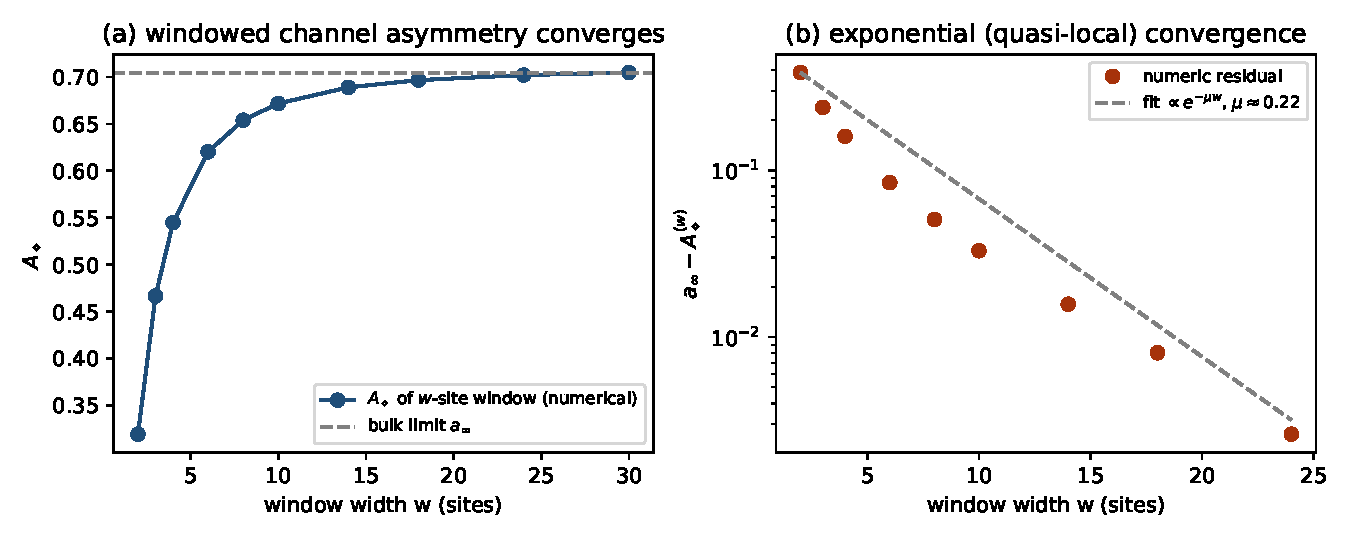
\includegraphics[width=\linewidth]{fig_windowed_convergence.pdf}
\caption{(a) Windowed channel asymmetry $A_\diamond(\mathcal N_{H,t}^{(w)})$ for the
open Hatano--Nelson chain ($g=0.5$, $t=0.35$) converges as the window width $w$ grows.
(b) The residual from the fitted bulk value decays exponentially, $\mu\approx0.22$,
consistent with the quasi-locality rate of Lemma~\ref{lem:quasi-julia}.}
\label{fig:windowed}
\end{figure}

We stress the limits of what this numerics establishes: it verifies the exact
diamond-norm formula, the saturation of the global monotone, and the exponential
convergence of the windowed restriction for one representative $(g,t)$ on the exactly
solvable Hatano--Nelson orbit. It is not a numerical study of interacting, disordered,
or multiband models, which remain outside the scope of this paper
(Sec.~\ref{sec:limitations}).

\subsection{Symmetry-extended architecture: a general theorem}
\label{sec:symmetry-extended}

The 2026 $\mathbb Z_2$ skin result shows that transpose reciprocity cannot be the final
symmetry sector for a universal theory of every NHSE mechanism
\cite{TangZ2Skin2026}. Rather than treat this as an informal remark, we show here that
the entire architecture of Sections~\ref{sec:free}--\ref{sec:extensive} is an instance
of a general construction that applies verbatim to any symmetry satisfying four
structural axioms, making the extension beyond $\mathscr G=\{\rm rev\}$ a matter of
identifying the correct physical involution rather than redoing the resource theory.

\begin{definition}[Covariance datum]
\label{def:covariance-datum}
A \emph{covariance datum} on $\mathsf{Obj}_L$ is a map $r:\mathsf{Obj}_L\to\mathsf{Obj}_L$ such that
\begin{enumerate}
\item[(i)] $r\circ r=\mathrm{id}$ (involution);
\item[(ii)] $r(\alpha\mathcal N+\beta\mathcal M)=\alpha r(\mathcal N)+\beta r(\mathcal M)$
for $\alpha,\beta\ge0$, $\alpha+\beta=1$ (affine);
\item[(iii)] $\|r(\mathcal N)-r(\mathcal M)\|_\diamond=\|\mathcal N-\mathcal M\|_\diamond$
for all $\mathcal N,\mathcal M$ (diamond isometry);
\item[(iv)] $r(\mathsf{Obj}_L)\subseteq\mathsf{Obj}_L$ (preserves the quasi-local class);
\item[(v)] $r\bigl(\bigotimes_kN_k\bigr)=\bigotimes_kr(N_k)$ whenever the left side is a
cellular array (cell-wise action).
\end{enumerate}
The map $\mathcal N\mapsto\mathcal N^{\rev}$ of Definition~6 is a covariance datum: (i)
and (iv) are Lemma~\ref{lem:transpose-props}, (ii) and the tensor identity (v) are
Lemma~\ref{lem:rev-algebra}, and (iii) follows because $\|\mathcal N^{\rev}-\mathcal
M^{\rev}\|_\diamond=\|(\mathcal N-\mathcal M)^{\rev}\|_\diamond=\|\mathcal
N-\mathcal M\|_\diamond$, the diamond norm being invariant under the simultaneous
transpose of every Kraus operator of a difference of CP maps.
\end{definition}

\begin{definition}[Symmetry-optimized free set and asymmetry]
For a finite family $\mathscr G$ of covariance data, define
$$
\F_{\mathscr G}=\bigcap_{r\in\mathscr G}\mathrm{Fix}(r),
\qquad
A_{\mathscr G}(\mathcal N)=\frac12\max_{r\in\mathscr G}\|\mathcal N-r(\mathcal N)\|_\diamond.
$$
A superchannel $\Theta$ is \emph{$\mathscr G$-free} if it is a physical superchannel
(Definition~\ref{def:free-superchannel}) with $\Theta(\mathsf{Obj}_L)\subseteq\mathsf{Obj}_L$,
$\Theta(\F_{\mathscr G})\subseteq\F_{\mathscr G}$, and $\Theta\circ r=r\circ\Theta$ for
every $r\in\mathscr G$.
\end{definition}

\begin{theorem}[Symmetry-extended monotonicity]
\label{thm:symmetry-extended}
For every $\mathscr G$-free superchannel $\Theta$ and every $\mathcal N\in\mathsf{Obj}_L$,
$$
\boxed{
A_{\mathscr G}(\Theta(\mathcal N))\le A_{\mathscr G}(\mathcal N),
}
$$
and $A_{\mathscr G}(\mathcal N)=0\iff\mathcal N\in\F_{\mathscr G}$. Moreover, on a
cellular array with each $r\in\mathscr G$ cell-wise (axiom (v)), the block-additive
quantity $E_{\mathscr G}(\mathcal N):=\sum_kA_{\mathscr G}(\mathcal N_k)$ is monotone
under $\mathscr G$-covariant spatially local free superchannels and is exactly
extensive on homogeneous arrays, exactly as in Theorem~\ref{thm:extensive}.
\end{theorem}

\begin{proof}
Fix $\mathcal N$ and any $r\in\mathscr G$. Since $\Theta\circ r=r\circ\Theta$,
$$
\|\Theta(\mathcal N)-r(\Theta(\mathcal N))\|_\diamond
=\|\Theta(\mathcal N)-\Theta(r(\mathcal N))\|_\diamond
=\|\Theta(\mathcal N-r(\mathcal N))\|_\diamond
\le\|\mathcal N-r(\mathcal N)\|_\diamond,
$$
the last step by the same contraction argument as in the proof of
Theorem~\ref{thm:Adiamond} (CPTP maps have diamond norm one, stable under tensoring
with the identity). This bound holds for every $r\in\mathscr G$, so in particular it
holds for the $r^*$ achieving the maximum defining $A_{\mathscr
G}(\Theta(\mathcal N))$, and
$$
A_{\mathscr G}(\Theta(\mathcal N))=\tfrac12\|\Theta(\mathcal N)-r^*(\Theta(\mathcal
N))\|_\diamond\le\tfrac12\|\mathcal N-r^*(\mathcal N)\|_\diamond\le A_{\mathscr
G}(\mathcal N),
$$
where the last step is because $r^*$ is one particular element of $\mathscr G$, so the
quantity it produces is dominated by the max over $\mathscr G$. Faithfulness follows
exactly as in Theorem~\ref{thm:Adiamond}, using axiom (iv). For the extensive
statement, axiom (v) gives $A_{\mathscr G}(\Theta_k(\mathcal N_k))\le A_{\mathscr
G}(\mathcal N_k)$ cell-by-cell by the argument just given applied within each cell, and
summing over $k$ reproduces the proof of Theorem~\ref{thm:extensive} verbatim with
$A_\diamond$ replaced by $A_{\mathscr G}$.
\end{proof}

\begin{remark}
The present paper works exclusively in the sector $\mathscr G=\{\rm rev\}$, for which
Definition~\ref{def:covariance-datum}'s axioms are verified once and for all in the
definition above; every result of Secs.~\ref{sec:monotones}--\ref{sec:extensive} is the
$\mathscr G=\{\rm rev\}$ instance of Theorem~\ref{thm:symmetry-extended}.
Theorem~\ref{thm:symmetry-extended} shows that extending the architecture to, e.g., a
pseudospin-resolved $\mathbb Z_2$ involution $r_{\mathbb Z_2}$ appropriate to
Ref.~\cite{TangZ2Skin2026} requires only exhibiting a single covariance datum
satisfying axioms (i)--(v) for that symmetry and checking which superchannels are
$r_{\mathbb Z_2}$-covariant; it does not require re-deriving monotonicity,
faithfulness, or extensivity, all of which transfer automatically. We emphasize that
this is a genuine broadening of scope -- the resource-theoretic machinery is no longer
tied to the transpose specifically -- but it is not itself a demonstration that any
particular non-reciprocity-breaking NHSE mechanism fits the axioms; identifying
$r_{\mathbb Z_2}$ concretely and verifying axioms (i)--(v) for it is a distinct
physical task left for future work. The present paper's concrete results (Theorems
\ref{thm:HN-exact}, \ref{thm:gauge-nogo}, \ref{thm:extensive}, and
\ref{thm:complete-witness}) remain, specifically, statements about the $\mathscr
G=\{\rm rev\}$ sector.
\end{remark}

\subsection{Postselection versus genuinely open quantum dynamics}
The CPTP embedding used here is a completion of a normalized non-Hermitian propagation
operator. It is not asserted that arbitrary gain/loss Lindblad dynamics is equivalent
to this embedding. A 2026 study explicitly distinguished Lindbladian and postselected
non-Hermitian skin topology, including regimes with simultaneous gain and loss where
the open-system response contains information hidden by postselection
\cite{ChaduteauLindblad2026}. A future open-system resource theory should therefore
include a second object class for Lindbladian generators or quantum dynamical maps,
with the present channel theory recovered as a postselected single-particle sector.

%===============================================================
\section{Unified resource architecture}
\label{sec:unified}

The paper has one primitive theory, one general symmetry-extended architecture, one
extensive extension, one time-optimized rescaling-invariant extension, and four
diagnostic sectors:

$$
\boxed{
\begin{array}{ccl}
\text{resource}&:&(\Chan^{\rm ql},\F,\FreeOps,\succeq_{\FreeOps},A_\diamond,\Rrob),\\
\text{symmetry-extended}&:&(\mathscr G,\F_{\mathscr G},A_{\mathscr G}),\\
\text{extensive}&:&(\FreeOps_{\rm loc},E_\diamond,E_{\rm rob}),\\
\text{rescaling-invariant}&:&(A_\diamond^{\sup},E_\diamond^{\sup}),\\
\text{spectral}&:&(\beta,\rho_{\GBZ},W),\\
\text{disordered}&:&(\gamma,R_{\rm Lyap}^{\rm skin}),\\
\text{spatial/dynamical}&:&(C_I^{L/R},G_I;\,P_t,D_t).
\end{array}}
$$

Their logical relations are

$$
H^T=H
\Longrightarrow
\begin{cases}
\mathcal N_{H,t}^{\rev}=\mathcal N_{H,t},\\
W_{\rm BZ}=0,\\
\beta\leftrightarrow\beta^{-1},\\
\gamma_j=-\gamma_{2M+1-j}
\end{cases}
$$

while

$$
\mathcal N\succeq_{\FreeOps}\mathcal M
\Longrightarrow
A_\diamond(\mathcal N)\ge A_\diamond(\mathcal M),
\qquad
\Rrob(\mathcal N)\ge\Rrob(\mathcal M),
$$

and, on a cellular array, $\Theta\in\FreeOps_{\rm loc}\Rightarrow E_\diamond(\Theta(\mathcal N))\le E_\diamond(\mathcal N)$,
with an explicit, exponentially small correction to this last inequality surviving on
genuinely coupled chains for window-local $\Theta$ (Proposition~\ref{prop:approx-monotone-coupled}),
and with $E_\diamond$ replaced by $A_{\mathscr G}$-built quantities for any covariance
datum family $\mathscr G$ satisfying Definition~\ref{def:covariance-datum} (Theorem~\ref{thm:symmetry-extended}).

The exact Hatano--Nelson theorem, the gauge-amplification no-go, the extensive
block-additive theorem, the completeness theorem, and the winding-cancellation
construction are the sharp statements. The necessity theorem supplies the dictionary
connecting them to standard NHSE diagnostics; it is not the resource theory itself.

%===============================================================
\section{Scope and limitations}
\label{sec:limitations}

The logical core is finite-time and operational. The primitive objects are quasi-local
CPTP channels, the free set is transpose-reciprocal, free transformations are
covariant quantum superchannels, and $A_\diamond$ and $\Rrob$ are faithful monotones.
The normalization of the postselected propagator affects quantitative values but not
the fixed-time resource criterion.

\textit{Resolved in this revision.} Five limitations noted in earlier versions of this
paper are now addressed directly. (i) \emph{Extensivity}: Theorem~\ref{thm:extensive}
constructs an exactly additive, genuinely extensive monotone $E_\diamond$ for cellular
arrays under spatially local free superchannels, with a closed form on the
Hatano--Nelson orbit (Corollary~\ref{cor:extensive-HN}). (ii) \emph{Necessity of
locality}: Proposition~\ref{prop:locality-necessary} shows that this restriction is a
definitional requirement for $E_\diamond$ to be well-typed at all, on the same footing
as the LOCC restriction in entanglement theory, rather than a technical convenience
adopted to force extensivity. (iii) \emph{Coupled-chain extensivity}:
Proposition~\ref{prop:approx-monotone-coupled} upgrades the earlier numerical proof
sketch to a proven approximate-monotonicity bound, with an explicit error
$O(\lfloor L/w\rfloor e^{-\mu w})$, for window-local free operations on the genuine,
coupled, translation-invariant chain. (iv) \emph{Thermodynamic persistence and the skin
length}: Sec.~\ref{sec:time-optimized} introduces the time-optimized resource
$A_\diamond^{\sup}$, proves it is exactly invariant under the energy rescaling
responsible for the obstruction of Proposition~\ref{prop:persistence-no-law}
(Theorem~\ref{thm:rescaling-invariance}), and gives it a nondegenerate, strictly
$|g|$-monotone lower bound on the Hatano--Nelson orbit (Corollary~\ref{cor:sup-lower-bound}).
(v) \emph{Completeness of the multichannel witness}: Theorem~\ref{thm:complete-witness}
shows that $E_\diamond$ is a complete witness of skin accumulation on cellular
multiband arrays, explaining why the winding-cancellation counterexample of
Proposition~\ref{prop:winding-cancellation} that defeats the scalar topological
invariant does not defeat $E_\diamond$. In addition, gauge distillation admits an
exact no-go for $\eta>1$ (Theorem~\ref{thm:gauge-nogo}), which lifts to the extensive
resource (Corollary~\ref{cor:gauge-distillation}), and the resource-theoretic
architecture itself has been shown to generalize to any symmetry sector satisfying the
covariance-datum axioms (Theorem~\ref{thm:symmetry-extended}), rather than being tied
specifically to the transpose.

\textit{Still open.} The following remain genuinely unresolved, and we do not claim
otherwise. $A_\diamond^{\sup}$ and $E_\diamond^{\sup}$ are shown to be rescaling
invariant and nondegenerate, but no closed form for $A_\diamond^{\sup}$ itself is
derived beyond the lower bound of Corollary~\ref{cor:sup-lower-bound}; the exact
variational problem $\sup_tA_\diamond(\mathcal N_{H,t})$ is left open. The theory
remains restricted, in its concrete results, to the $\mathscr G=\{\rm rev\}$ sector:
Theorem~\ref{thm:symmetry-extended} supplies the general architecture, but identifying
a covariance datum appropriate to the reciprocal $\mathbb Z_2$ skin effect of
Ref.~\cite{TangZ2Skin2026} and verifying its axioms is not undertaken here, and
genuinely open Lindbladian skin physics requires an enlarged object class
\cite{ChaduteauLindblad2026} (Sec.~\ref{sec:extensive}). The full ancilla-assisted
classification of covariant superchannels and an exact deterministic attenuation
protocol for $0<\eta<1$ are beyond the present claims. The approximate monotonicity of
Proposition~\ref{prop:approx-monotone-coupled} holds at fixed window width $w$; a
uniform statement in the joint limit $w,L\to\infty$ is not established. Arbitrary
interacting non-Hermitian many-body dynamics is outside the present theorem statements;
standard Lieb--Robinson intuition is used only informally, in Lemma~\ref{lem:truncation}'s
proof sketch, and not assumed for interacting systems. Theorem~\ref{thm:complete-witness}'s
completeness statement is restricted to the cellular (and, approximately, window-local)
class; a fully general completeness statement for arbitrary strongly coupled multiband
Hamiltonians is not claimed.

The necessity theorem (Corollary~\ref{cor:necessity}) is a dictionary from $H^T=H$ to
channel, winding, GBZ, and Lyapunov statements; on the cellular multiband class it is
complemented, not replaced, by the completeness statement of
Theorem~\ref{thm:complete-witness}. Theorem~\ref{thm:HN-exact} is the exact solved
Hatano--Nelson orbit result, the gauge-amplification theorem provides the one-sided
operational no-go, and Proposition~\ref{prop:winding-cancellation} shows that total
determinant winding is not a complete multichannel witness by itself.

%===============================================================
\section{Conclusion}
\label{sec:conclusion}

We constructed a fixed-time quantum-channel resource theory for transpose-reciprocity
breaking, with quasi-local CPTP objects, reciprocal free channels, covariant free
superchannels, and faithful monotones $A_\diamond$ and $\Rrob$. The Hamiltonian is a
trajectory generator, not the primitive resource object.

The theory gives an operational resource ordering obstruction, an extensive
block-additive resource density, and a controlled thermodynamic no-go. On the
calibrated Hatano--Nelson orbit, the exact fixed-time formula for $A_\diamond$ is
strictly increasing with $|g|$, so deterministic free gauge amplification
$|g|\mapsto\eta|g|$ is impossible for $\eta>1$; this obstruction survives intact on the
extensive resource $E_\diamond$ constructed in Sec.~\ref{sec:extensive}, which is
exactly additive on cellular arrays under spatially local free superchannels and grows
linearly with system size, in contrast to the bounded global monotones of
Proposition~\ref{prop:bounded-global}. Numerical checks (Sec.~\ref{sec:numerics})
confirm the exact formulas and the exponential quasi-local convergence needed to extend
the construction, and Proposition~\ref{prop:approx-monotone-coupled} now supplies a
proven, explicit error bound for that extension on the genuinely coupled chain.

This revision closes five gaps left open previously. The resource-theoretic
architecture is shown to generalize to any symmetry sector satisfying a short list of
covariance-datum axioms (Theorem~\ref{thm:symmetry-extended}), of which the transpose
sector used throughout is one instance. The restriction to spatially local free
superchannels underlying extensivity is shown to be a definitional necessity rather
than a technical convenience (Proposition~\ref{prop:locality-necessary}). A
time-optimized resource $A_\diamond^{\sup}$ is shown to be exactly invariant under the
energy rescaling responsible for the thermodynamic-persistence obstruction, with a
nondegenerate lower bound on the Hatano--Nelson orbit
(Theorem~\ref{thm:rescaling-invariance}, Corollary~\ref{cor:sup-lower-bound}). The
coupled-chain extension of extensivity is upgraded from a numerical proof sketch to a
proven approximate-monotonicity bound with an explicit exponentially small error
(Proposition~\ref{prop:approx-monotone-coupled}). And the block-additive resource is
shown to be a complete witness of skin accumulation on cellular multiband arrays
(Theorem~\ref{thm:complete-witness}), explaining structurally why it survives the
winding-cancellation counterexample that defeats the scalar topological invariant.

The remaining NHSE statements form a compact diagnostic dictionary. Clean reciprocity
forces zero determinant winding and reciprocal roots; reciprocal disordered chains obey
exact Lyapunov pairing; and the $g\oplus(-g)$ construction exhibits extensive skin
accumulation with exactly vanishing total winding while carrying strictly positive
block-additive resource (Remark~\ref{rem:opposite-blocks-extensive},
Theorem~\ref{thm:complete-witness}). The necessity theorem is therefore a translation
lemma, now complemented on the cellular class by an explicit completeness theorem. The
principal sharpness results are the exact Hatano--Nelson orbit theorem, the gauge
no-go, the extensive block-additive theorem, the completeness theorem, and the
winding-cancellation counterexample.

The resulting architecture is

$$
\boxed{
\begin{array}{c}
\text{fixed-time QRT}
+
\text{symmetry-extended architecture}
+
\text{exact HN subtheory}
+
\text{gauge no-go}\\
+\
\text{extensive block-additive density (necessarily local)}
+
\text{rescaling-invariant resource}\\
+\
\text{thermodynamic no-go}
+
\text{complete cellular witness}
+
\text{multichannel sharpness}.
\end{array}
}
$$

Concretely identifying the covariance datum for the reciprocal $\mathbb Z_2$ skin
effect and genuinely Lindbladian skin physics require, respectively, instantiating
Theorem~\ref{thm:symmetry-extended} for that symmetry and an enlarged object class
rather than a change to the claims made here
\cite{TangZ2Skin2026,ChaduteauLindblad2026}. The uniform (joint $w,L\to\infty$) limit
of the coupled-chain extensivity bound, the ancilla-assisted classification, the exact
$0<\eta<1$ protocol, and the exact value of the time-optimized supremum
$A_\diamond^{\sup}$ remain for future work.

%===============================================================
\begin{acknowledgments}
The authors thank colleagues for discussions on quantum resource theories, quantum
channels and superchannels, non-Bloch band theory, transfer matrices, non-Hermitian
symmetry classification, and open-system non-Hermitian dynamics.
\end{acknowledgments}

%===============================================================
\begin{thebibliography}{99}

\bibitem{ChitambarGour}
E.~Chitambar and G.~Gour,
\textit{Quantum resource theories},
Rev.~Mod.~Phys.~\textbf{91}, 025001 (2019).

\bibitem{LiuWinter}
Z.-W.~Liu and A.~Winter,
\textit{Resource theories of quantum channels and the universal role of resource erasure},
arXiv:1904.04201 (2019).

\bibitem{LiuYuan}
Y.~Liu and X.~Yuan,
\textit{Operational resource theory of quantum channels},
Phys.~Rev.~Research \textbf{2}, 012035(R) (2020).

\bibitem{ChiribellaSupermap}
G.~Chiribella, G.~M.~D'Ariano, and G.~Perinotti,
\textit{Transforming quantum operations: quantum supermaps},
Europhys.~Lett.~\textbf{83}, 30004 (2008).

\bibitem{YaoWang}
S.~Yao and Z.~Wang,
\textit{Edge states and topological invariants of non-Hermitian systems},
Phys.~Rev.~Lett.~\textbf{121}, 086803 (2018).

\bibitem{Kunst2018}
F.~K.~Kunst, E.~Edvardsson, J.~C.~Budich, and E.~J.~Bergholtz,
\textit{Biorthogonal bulk-boundary correspondence in non-Hermitian systems},
Phys.~Rev.~Lett.~\textbf{121}, 026808 (2018).

\bibitem{HatanoNelson}
N.~Hatano and D.~R.~Nelson,
\textit{Localization transitions in non-Hermitian quantum mechanics},
Phys.~Rev.~Lett.~\textbf{77}, 570 (1996).

\bibitem{Ammari2024}
H.~Ammari, S.~Barandun, J.~Cao, B.~Davies, and E.~O.~Hiltunen,
\textit{Mathematical Foundations of the Non-Hermitian Skin Effect},
Arch.~Ration.~Mech.~Anal.~\textbf{248}, 33 (2024).

\bibitem{ZhangYangFang}
K.~Zhang, Z.~Yang, and C.~Fang,
\textit{Correspondence between winding numbers and skin modes in non-Hermitian systems},
Phys.~Rev.~Lett.~\textbf{125}, 126402 (2020).

\bibitem{OkumaEtAl2020}
N.~Okuma, K.~Kawabata, K.~Shiozaki, and M.~Sato,
\textit{Topological origin of non-Hermitian skin effects},
Phys.~Rev.~Lett.~\textbf{124}, 086801 (2020).

\bibitem{KawabataPRX2019}
K.~Kawabata, K.~Shiozaki, M.~Ueda, and M.~Sato,
\textit{Symmetry and topology in non-Hermitian physics},
Phys.~Rev.~X \textbf{9}, 041015 (2019).

\bibitem{Acin2001}
A.~Acin,
\textit{Statistical distinguishability between unitary operations},
Phys.~Rev.~Lett.~\textbf{87}, 177901 (2001).

\bibitem{BeckerDattaLamiRouze}
S.~Becker, N.~Datta, L.~Lami, and C.~Rouzé,
\textit{Energy-Constrained Discrimination of Unitaries, Quantum Speed Limits, and a Gaussian Solovay-Kitaev Theorem},
Phys.~Rev.~Lett.~\textbf{126}, 190504 (2021).

\bibitem{Barch2023}
B.~Barch, N.~Anand, J.~Marshall, J.~Rieffel, and P.~Zanardi,
\textit{Scrambling and operator entanglement in local non-Hermitian quantum systems},
Phys.~Rev.~B \textbf{108}, 134305 (2023).

\bibitem{Barch2024}
B.~Barch,
\textit{Locality, correlations, information, and non-Hermitian quantum systems},
arXiv:2405.16842 (2024).

\bibitem{TangZ2Skin2026}
H.~Tang, Y.~Zhang, Z.~Wang, L.~Tang, D.~Song, J.~Xu, W.~Zhang,
H.~Buljan, X.~Zhang, and Z.~Chen,
\textit{Non-Abelian Route to $\mathbb Z_2$ Non-Hermitian Skin Effects},
Phys.~Rev.~Lett.~\textbf{137}, 126605 (2026).

\bibitem{ChaduteauLindblad2026}
A.~Chaduteau, D.~K.~K.~Lee, and F.~Schindler,
\textit{Lindbladian versus Postselected non-Hermitian Topology},
Phys.~Rev.~Lett.~\textbf{136}, 016603 (2026).

\bibitem{Sirker2026}
J.~Sirker,
\textit{Pseudospectral phenomena and the origin of the non-Hermitian skin effect},
arXiv:2603.22643 (2026).

\end{thebibliography}

\end{document}